% IDSC LaTeX Thesis Template
% 
% Author(s):	Eric Müller
% 				Institute for Dynamic Systems and Control
% 				Swiss Federal Institute of Technology (ETH) Zurich
% 
% Created:		2004/04/02  (Eric Mueller)
% 
% Notes: Has been tested on Windows 7 + MikTeX + TeXnicCenter
%
% Revisions: 	2009/05/29  (Soren Ebbesen)
% 				    2011/03/22	(Soren Ebbesen)
%             2013/03/08	(Soren Ebbesen)
%             2014/03/13	(Soren Ebbesen)
% ______________________________________________________________________________
\documentclass[10pt,twoside,a4paper,fleqn]{report}


\usepackage[english,st]{ethidsc} % Special IDSC styles and commands      	
								 % {german}/english: language of headings, etc.
								 % {st}/bt/mt: {semester}/bachelor/master thesis
							
% Page header (don't change)____________________________________________________
\setlength{\parindent}{0em}                 % Disable parindent
\rhead[\nouppercase{\rightmark}]{\thepage}  % Special headings
\lhead[\thepage]{\nouppercase{\leftmark}}   % Special headings
\cfoot{}                                    % Special headings


% Title page (please fill in)___________________________________________________
\title{CUBLI Choreographer}


\studentA{Daniel Dugas}
\ethidA{11-830-429}
\semesterA{5}
\emailA{dugasd@student.ethz.ch}

%\studentB{Second Student}
%\ethidB{12-345-678}
%\semesterB{9}
%\emailB{second@student.ethz.ch}

\supervision{Michael M\"uhlebach}
\date{August 2015}

\identification{IDSC-RD-MMu-03} 		% Project identifier

\infopage
\declaration

% Begin document________________________________________________________________
\begin{document}

\maketitle 							% Create title page


% Preamble______________________________________________________________________

\pagenumbering{roman} 				% Begin roman page numbering (i,ii,...)

%---------------------------------------------------------------------------
% Preface

% \chapter*{Preface}

% Blah blah \dots

% \cleardoublepage

%---------------------------------------------------------------------------
% Table of contents

 \setcounter{tocdepth}{2}
 \tableofcontents

 \cleardoublepage

%---------------------------------------------------------------------------
% Abstract

\chapter*{Abstract}
 \addcontentsline{toc}{chapter}{Abstract}

This Semester Project devises and implements a way of controlling one or several Cublis wirelessly.\\ 

Cublis are cube-shaped, balancing robots developed at the IDSC lab in ETH Zurich, which have the peculiarity of being controlled by inertial reaction wheels inside the structure. As such, they are able to have no exterior moving parts, while still being able to jump, balance on corners and edges, and even spin.\\ 

Cubli robots are currently controlled using button-presses on the robot hardware itself. Upon successful completion of this project, a user will be able to send and receive commands to/from Cubli using a specific interface created during the course of the project.\\

The interface is developed as a computer application, presenting on the user with tools for creating a choreography - that is, a sequence of actions a cubli should perform, - running, and stopping it.\\ 

The application then communicates wirelessly with one or several cublis in order to have them execute those actions. In order to achieve that, a custom communication protocol is created, allowing the cubes and computer to transfer data to each other via serial port.\\ 

An intended consequence of this interface and protocol, is that the implementation of the above opens up further possibilities in several directions, for later projects. 
For example, since this implements a way for cubli to send, receive, and interpret messages, it leads to the possibility of making cublis interact with each other, in the sense of working together responsively in any scenario, not just in a choreography.
The fact that cubli's interface is now augmented also means that it would be simpler to implement complex behaviors such as moving around in any direction through consecutive jumps, or balancing on arbitrary corners.\\

By creating and using the Cubli and its interface, real behavior can be compared to theory. Thus the feasability of further endeavors can be assessed, as well as the particular aspects which present challenges or show promise.

 \cleardoublepage


%---------------------------------------------------------------------------

% Chapters______________________________________________________________________

\pagestyle{fancy}               	% Fancy headings
\pagenumbering{arabic}				% Begin arabic page numbering (1,2,...)

\chapter{Introduction}\label{sec:introduction}

\section{The IDSC Cubli}\label{sec:cubli}

\begin{figure}[ht]
   \centering
   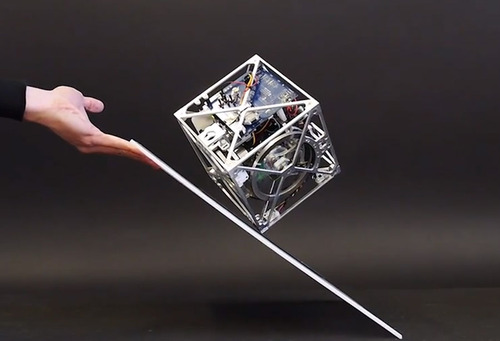
\includegraphics[width=0.75\textwidth]{img/Cubli.jpg}
   \caption{The IDSC Cubli balancing on a slanted surface.}
   \label{img:Cubli}
\end{figure}

The Cubli is a robotic cube developed at the IDSC lab in ETH Zurich, with the ability to balance on its edges and corners by using internal reaction wheels. Of relatively small size, that is dimensions of 15 x 15 x 15 cm, the robot is a proof-of-concept made possible through innovative design and engineering.\\

On top of its ability to balance, Cubli is also able to jump through well-timed braking of the reaction wheels. It can thus jump from a face to an edge, a corner, or from a face directly to the corner. It is also able to spin, and stop spinning when balancing on a corner.

\begin{figure}[ht]
   \centering
   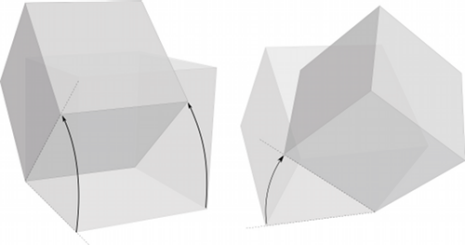
\includegraphics[width=0.75\textwidth]{img/Jumps.png}
   \caption{Illustration of Cubli's jumping abilities.}
   \label{img:Jumps}
\end{figure}

\subsection{Original Interface}

Actions can be executed by pressing buttons visible on one of cubli's faces ( \textit{See Figure \ref{img:Buttons}} ). For example, pressing the Mode button once while holding cubli on its edge at a stable angle will cause it to start balancing. Or, when cubli is on its face, press the mode button once and it jumps up to its edge.\\

\begin{figure}[ht]
   \centering
   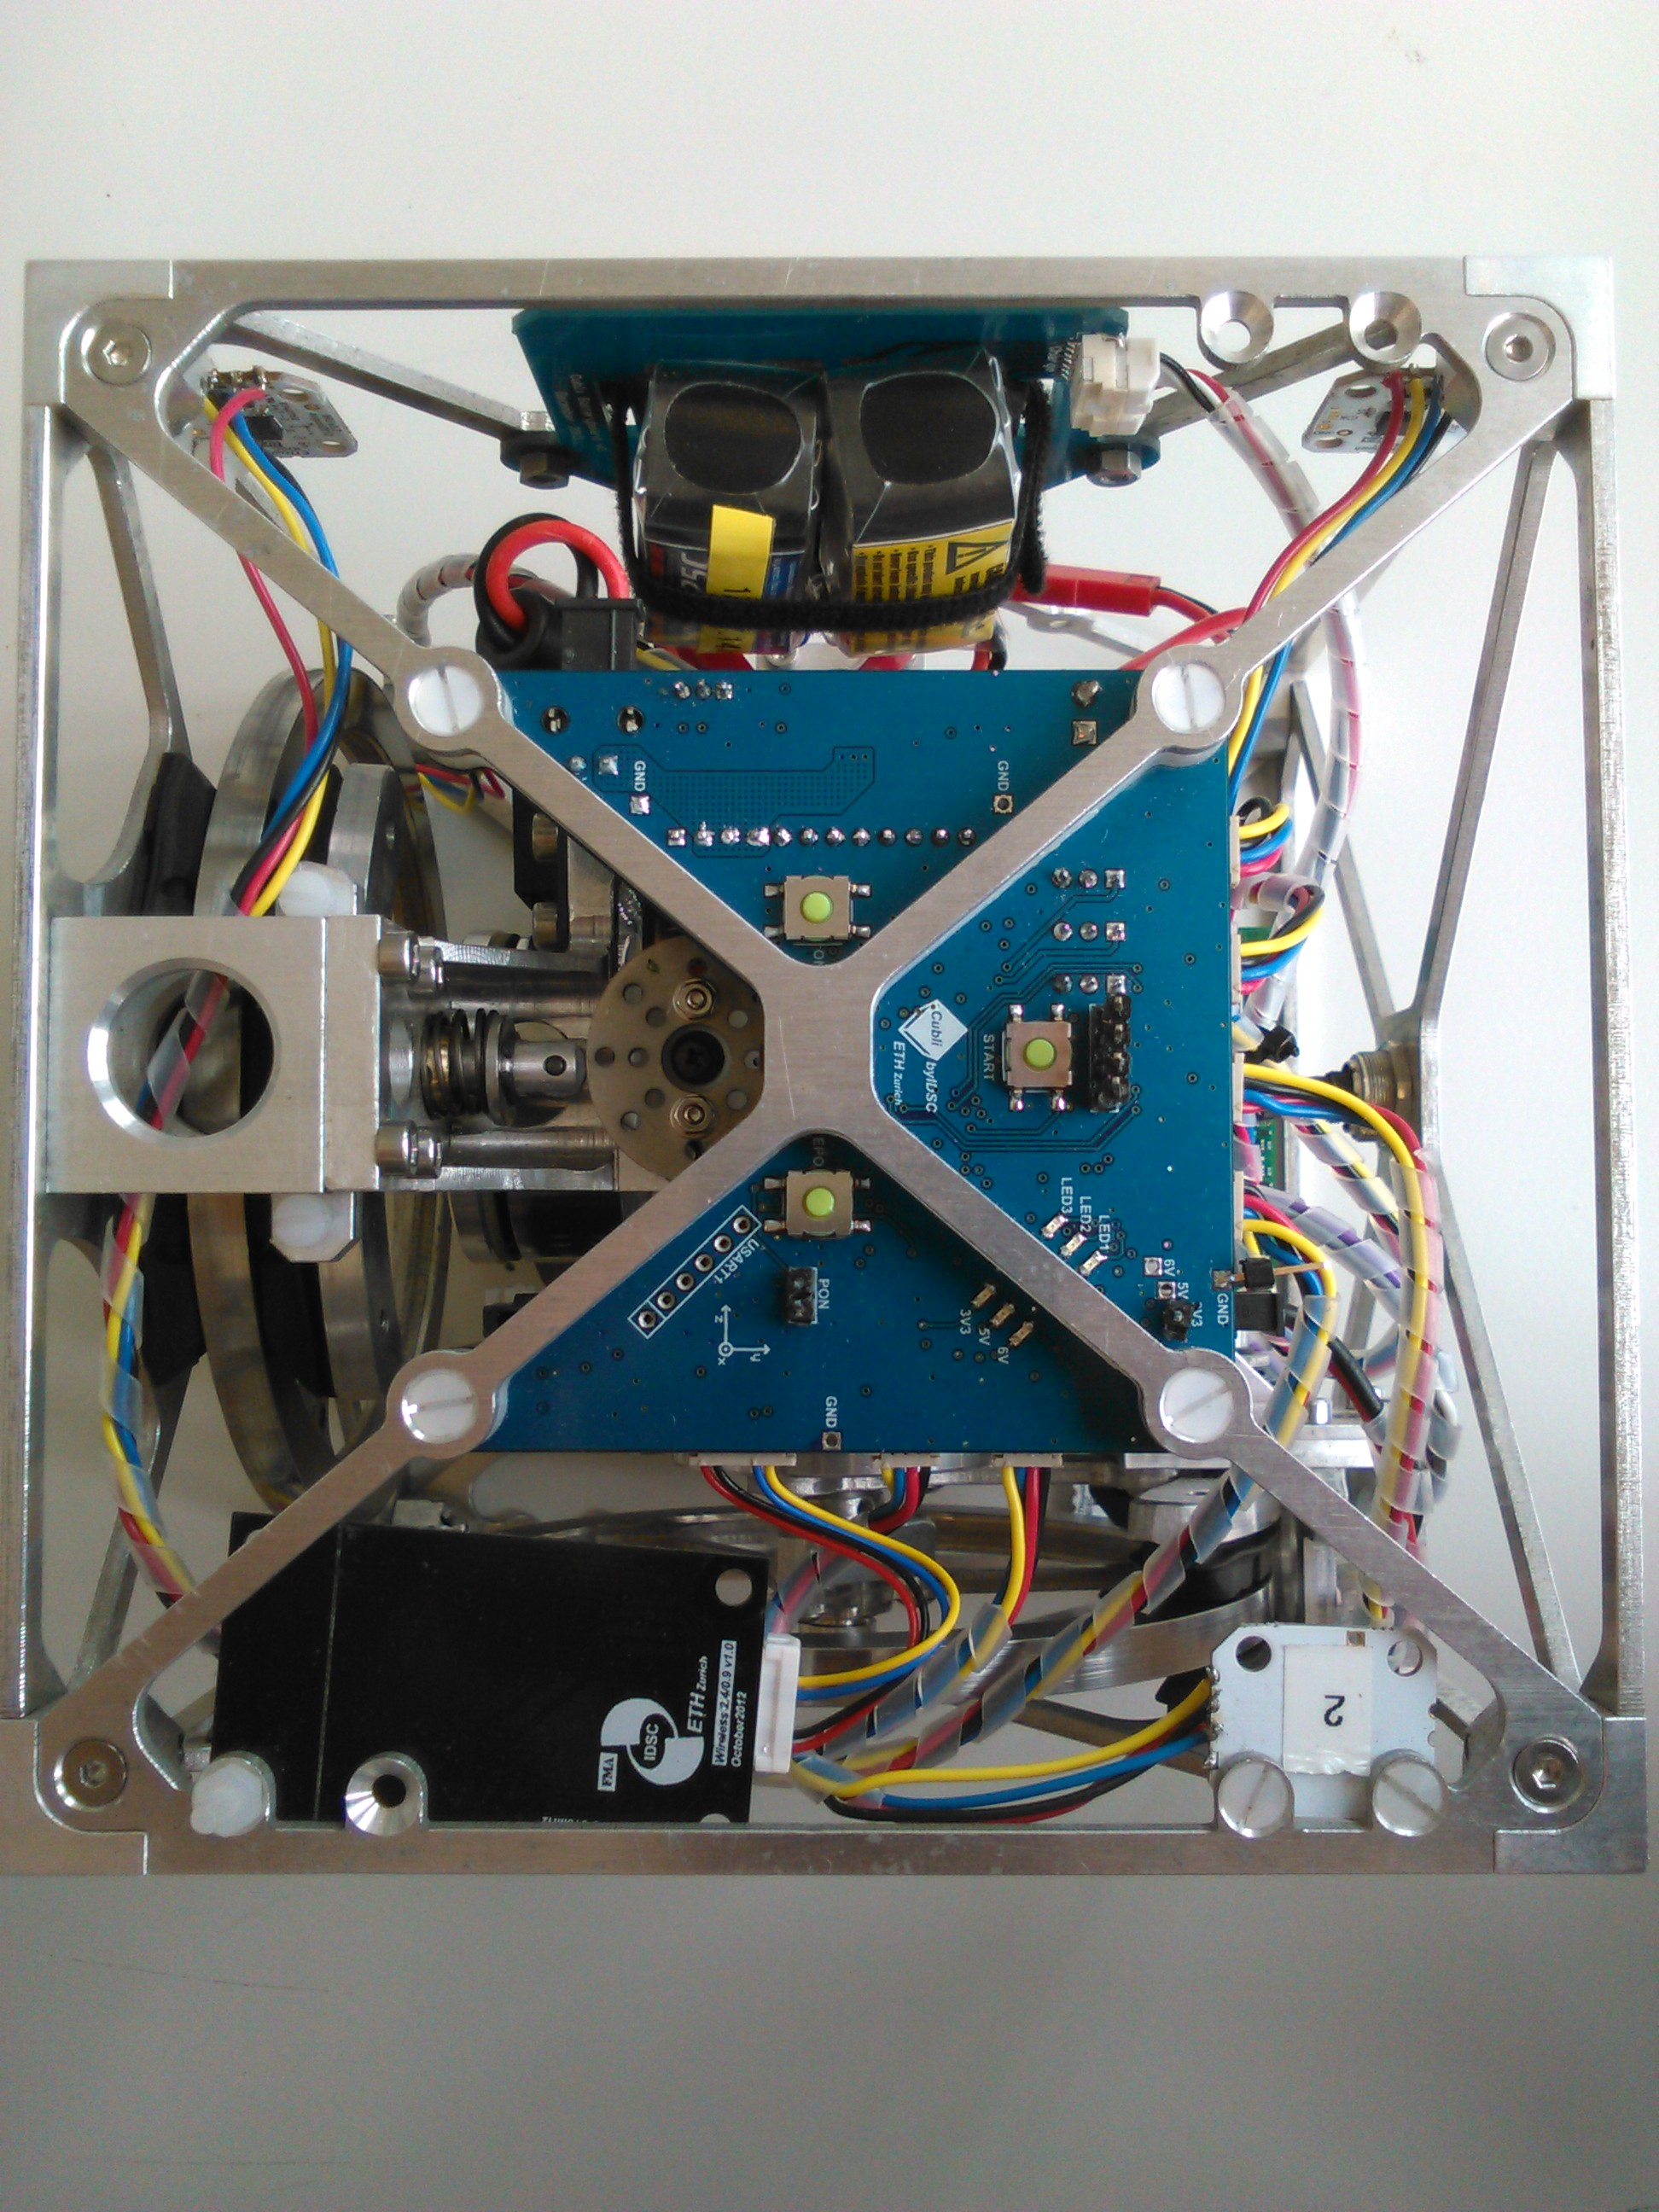
\includegraphics[width=0.75\textwidth]{img/Buttons.jpg}
   \caption{The three buttons on Cubli's controller, used to interact with cubli.}
   \label{img:Buttons}
\end{figure}

Though this is a very reliable interface, it can present inefficiencies. For example, it is sometimes desirable to press the mode button when cubli is balancing, in order to have it perform an action. However, doing so upsets cubli's balance, since pressing a button implies exerting a force on cubli's exterior.\\

This project's proposition is to offer an alternate interface, without removing the already existing one - the buttons shall still serve their original functions. Controlling cubli from a nearby device presents interesting challenges and possibilities, thus making for a promising aim.

\subsection{Original Communications Abilities}

Before the project was started, Cubli was already fitted with a wireless communication device, set up for one-way communication from cubli to computer, for debugging and supervision purposes.\\

\begin{figure}[ht]
   \centering
   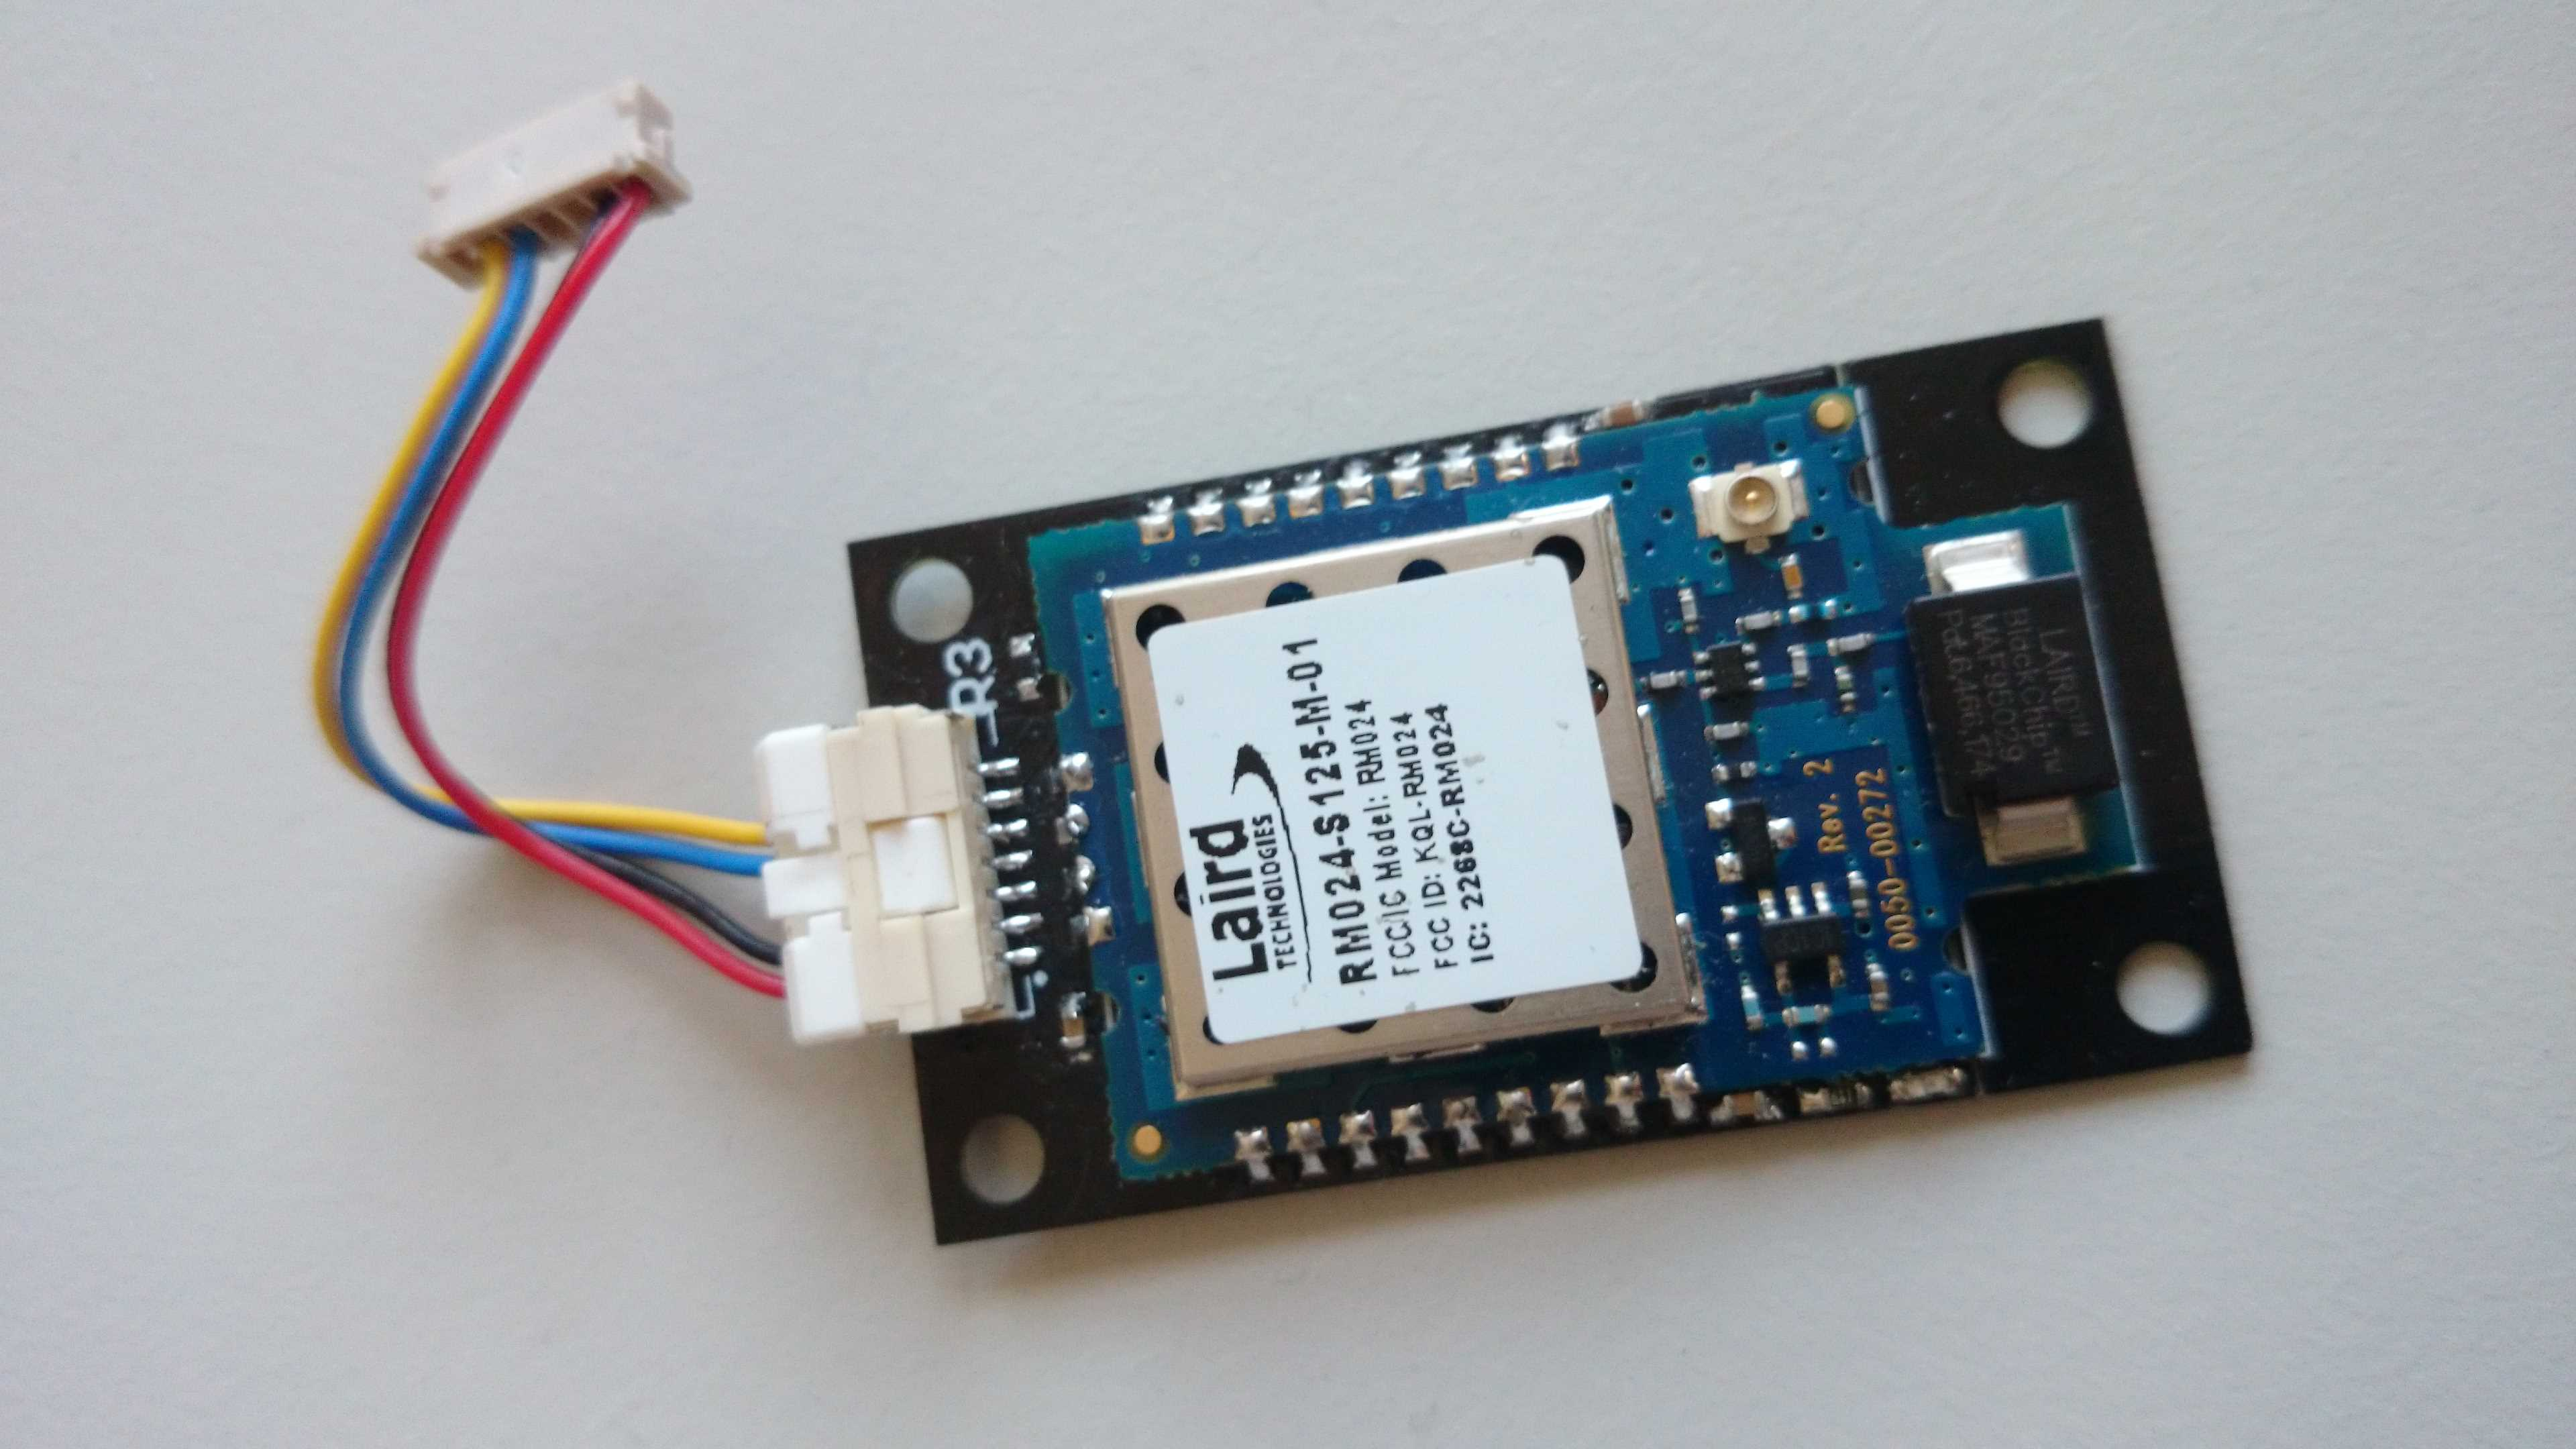
\includegraphics[width=0.75\textwidth]{img/LAIRD-radio.jpg}
   \caption{Radio used in the Cubli hardware.}
   \label{img:LAIRD-radio}
\end{figure}

As such it made sense to consider developping two-way communications using the already-present hardware, and the potential applications of this modification.\\ 

Because physical interaction with the robot generally hinders its ability to balance and move freely, wireless communication is a desired part of the new interface's implementation.
Yet it is even more important than that.\\

The project aims to extend the interface, but also to test Cublis ability not only to simply receive commands from the user, but also to communicate in a multilateral fashion. That is, to set the basis for smarter Cublis that can exchange information, and display responsive behavior. 

\section{Project Goals}

As the previous section outlines the original capabilities of Cubli, and how the project is in general going to affect them, this section lays out the practical implementation which is sought. This implementation is meant to showcase the properties ( some of which were expressed previously ) which are:
\begin{enumerate}
\item augmented interface
\item responsiveness
\item multiple cubli coordination
\item further feature potential.
\end{enumerate}

Thus the Cubli choreographer concept was created: An interface allowing not only for wireless control of a Cubli, but also allowing for the introduction of more independent and responsive behavior.\\

By giving the robot not straightforward commands, but more complex sequences which it needs to store and perform - acting autonomously to ensure the correct proceeding of those sequences, and reacting to failures - the interface delegates agency to the cube.\\

In addition, the choreographer shall be designed to interact with several cublis at once, coordinating their actions.\\

Thus, should the concept be proved to be realizable, it will effectively showcase the desired properties outlined in the previous paragraph.




\cleardoublepage
\chapter{Specifications}\label{sec:specifications}

The initial task of the project was to define the project goals and specifications, and the basic structure of the development plan.\\ 

Thinking of the necessary components and the actions which would be required of them in order to generate the desired behavior, it was clear that at the minimum the project would require two separate programs, and thus at least two code bases. In addition, acting as a bridge within the two, and since it would likely be a quite significant endeavor in itself, the communication code was also separated conceptually and is discussed in the following as such.\\ 

 From this understanding, development is split into three main modules :

\begin{enumerate}
\item App behavior implementation - User Experience (C++)  
\item Communications implementation  (C++/C)
\item Cubli behavior implementation  (C)  
\end{enumerate}
 
Which can be described as follows:

\subsubsection{App Behavior Implementation}

The choreographer application has to be designed from scratch, providing an efficient and reliable way for users to interact wirelessly with the cubli. \\

One of the main objectives when designing the interface was for it to be as simple and intuitive as possible.
 
\subsubsection{Communications Implementation}

Acting as a bridge between the cubli and choreographer source code, the communications protocol behavior has to match in both cases, allowing messages encrypted in one to be decrypted by the other.

\begin{description}
\item[] Desired specifications for the protocol :
\begin{description}
  \item[Robust] - Ensuring that messages are transmitted successfully, and    strict prevention of information corruption in the process. 

  \item[Lightweight] - Minimal amount of processor overhead in order to not disrupt other tasks in cubli 

  \item[Concise] - Making messages as short as possible while ensuring that 	any information which needs to be transferred can be conveyed using the 	protocol. 

  \item[Cross-compatible] - Ensuring that the code could be compiled on the 	two other modules and would yield the same behavior (c.f. signedness 	issues) 
\end{description}
\end{description}
 
\subsubsection{Cubli Behavior Implementation}

Having received information representing the choreography description, status of other cubes, or user commands, the cubli has to react accordingly.

Pre-existing cubli source code had to be supplemented and modified to implement the expected behavior.




\section{User Interface}

The goal is to create the choreographer application, an easy to launch and use executable.

Its specified core functionalities are:

\begin{itemize}
\item Choreography creation, and following that, modification
\item Choreography execution and control
\item Real-time display of choreography status
\item Real-time display of cubli status
\end{itemize}

along with the implied necessary functionalities:

\begin{itemize}
\item Communication with Cubli, and optionally display of those communications
\item Options for setting up the serial port
\end{itemize}


The application itself could in theory take many forms and still satisfy the necessary functionality. In order to decide which direction to take, examples of existing implementations were considered. These examples are applications with uses unrelated to the cubli choreographer, but which contain UI aspects that fulfill similar requirements as the ones pertaining to the choreographer application.\\

As an example, it would be possible to satisfy all those functionalities in a command-line interface ( \textit{c.f. Figure \ref{img:CommandLine}} ) . However, ease of use and simplicity go out the window in such an implementation when it comes to the timeline creation process. For that reason particularly, a graphical user interface, although it requires longer and more complex development, was deemed optimal.\\

\begin{figure}[ht]
   \centering
   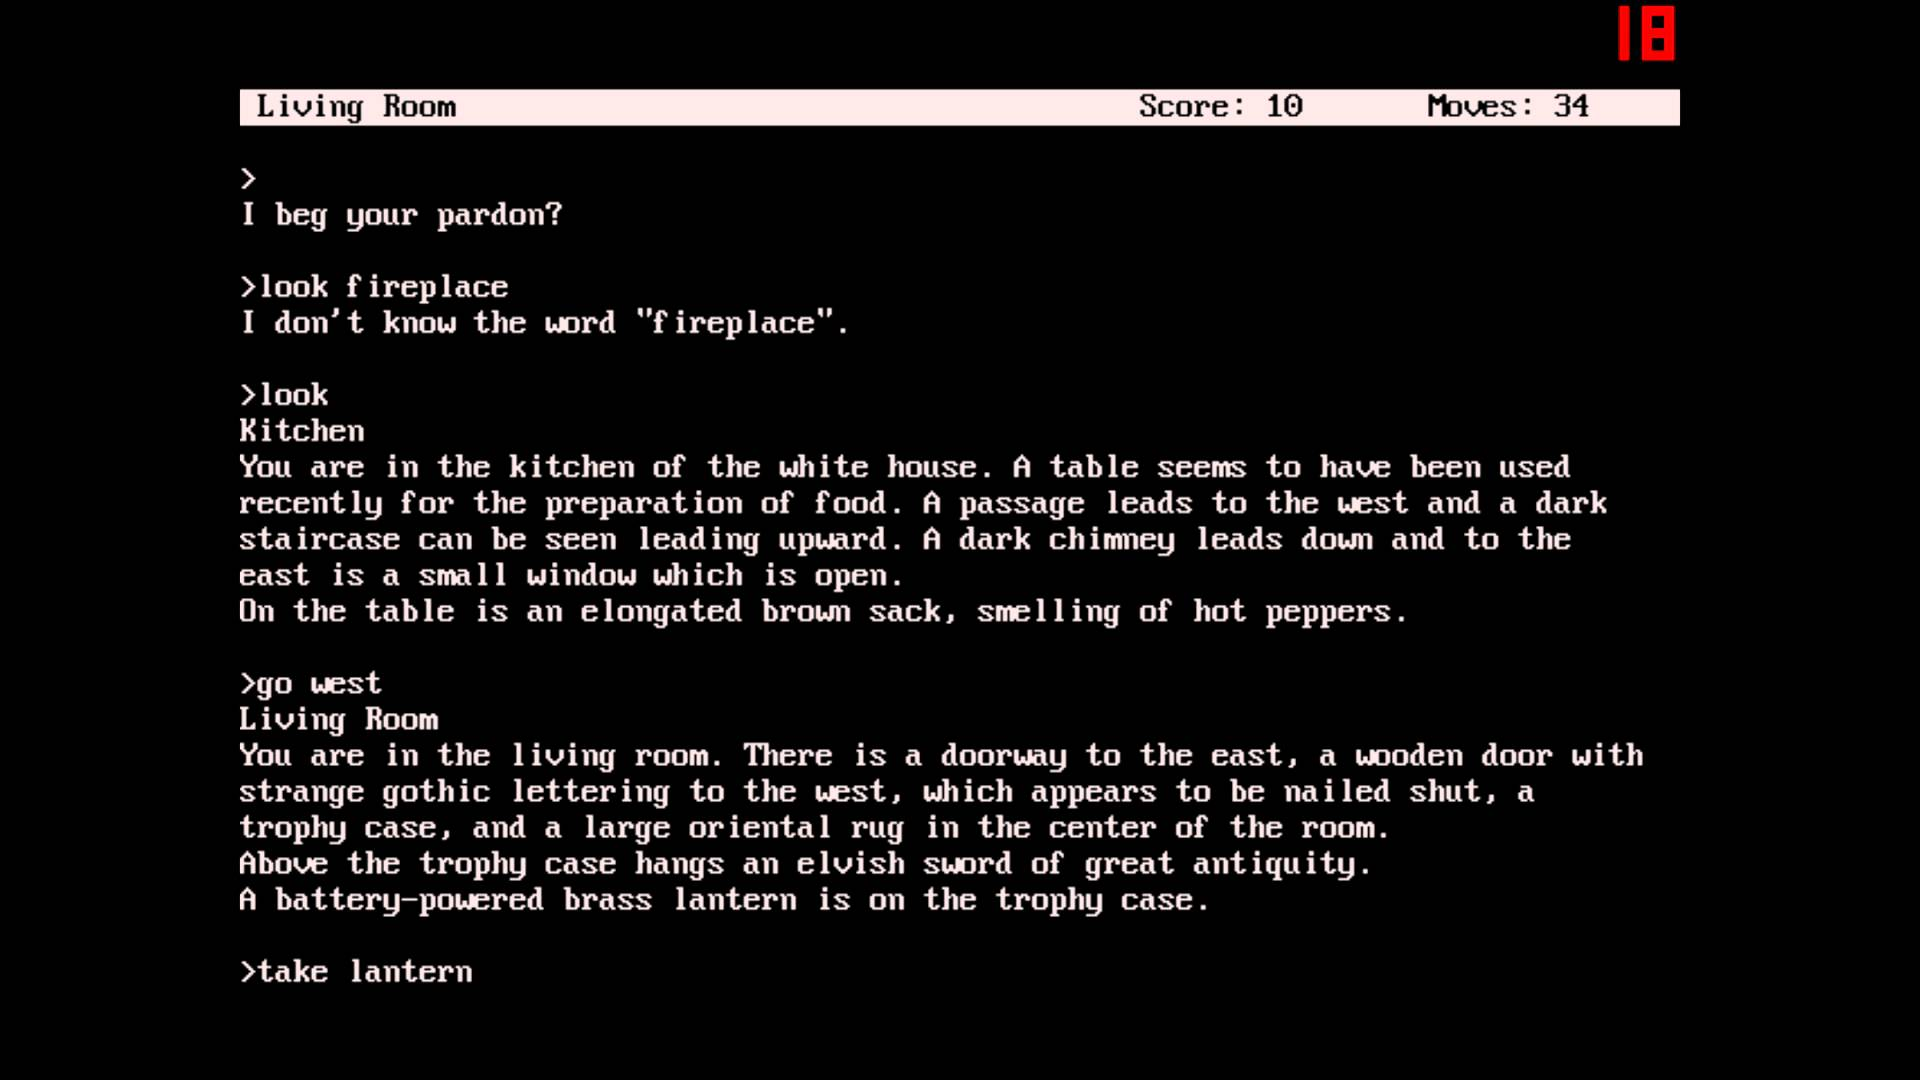
\includegraphics[width=0.75\textwidth]{img/CommandLine.jpg}
   \caption{Command-line interfaces can be used for many purposes.}
   \label{img:CommandLine}
\end{figure}

In fact, since the creation process lies at the center of the choreographer concept, and due to the other functionalities requiring little screen space in comparison, it makes sense for the choreography creation interface to occupy most of the interface, and dictate many design decisions.\\

Remaining functionalities to fulfill would be choreography control, port and application settings, extra user information and communication display.\\

In designing the interface, the parallel was made media music applications since the idea of a choreography can be conceptually tied with music. This applies in particular to the choreography control interface ( \textit{c.f. Figure \ref{img:GoogleMusic}} ).\\

\begin{figure}[ht]
   \centering
   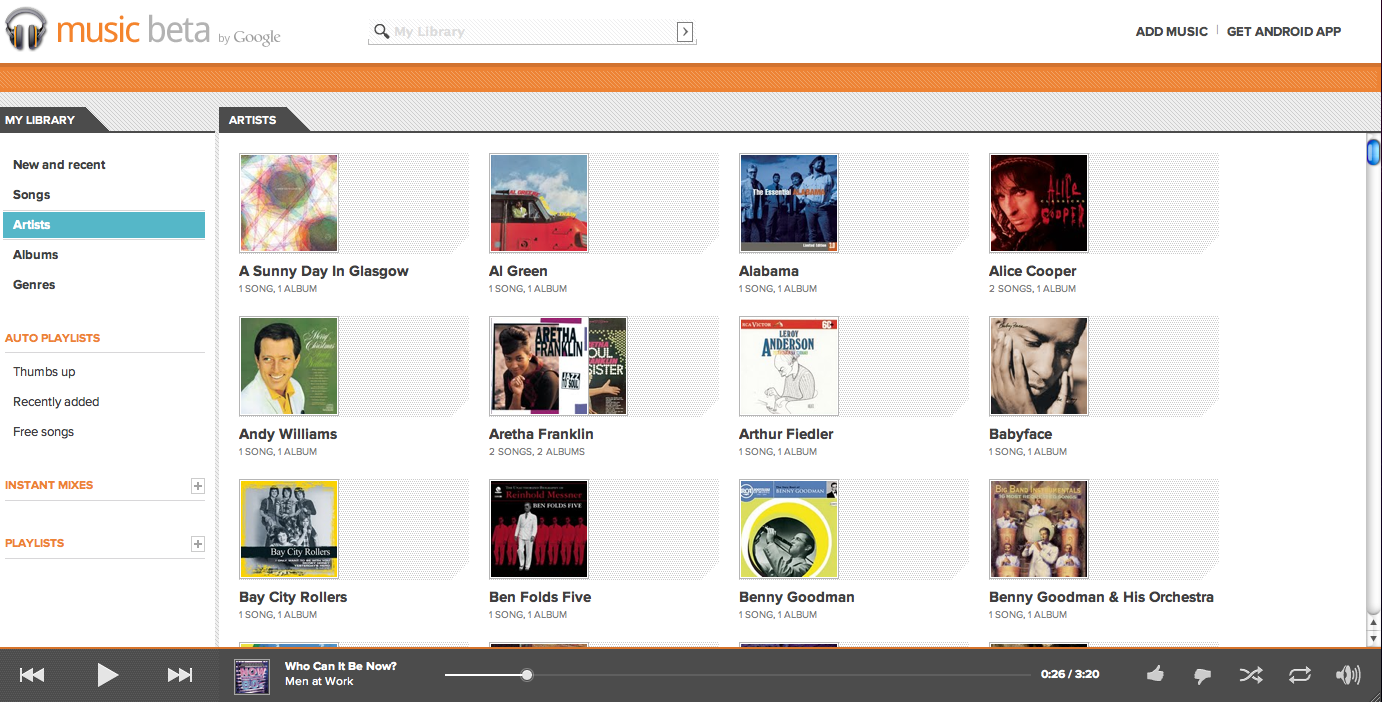
\includegraphics[width=0.75\textwidth]{img/GoogleMusic.png}
   \caption{Example of music player. Relevant are the simple controls at the bottom.}
   \label{img:GoogleMusic}
\end{figure}

In a similar vein, music or video creation/splicing softwares often deal with similar manipulation of time-dependent sequences by the user, and their solutions are particularly suited to the purposes of this project ( \textit{c.f. Figure \ref{img:MusicEditor}} ).\\

\begin{figure}[ht]
   \centering
   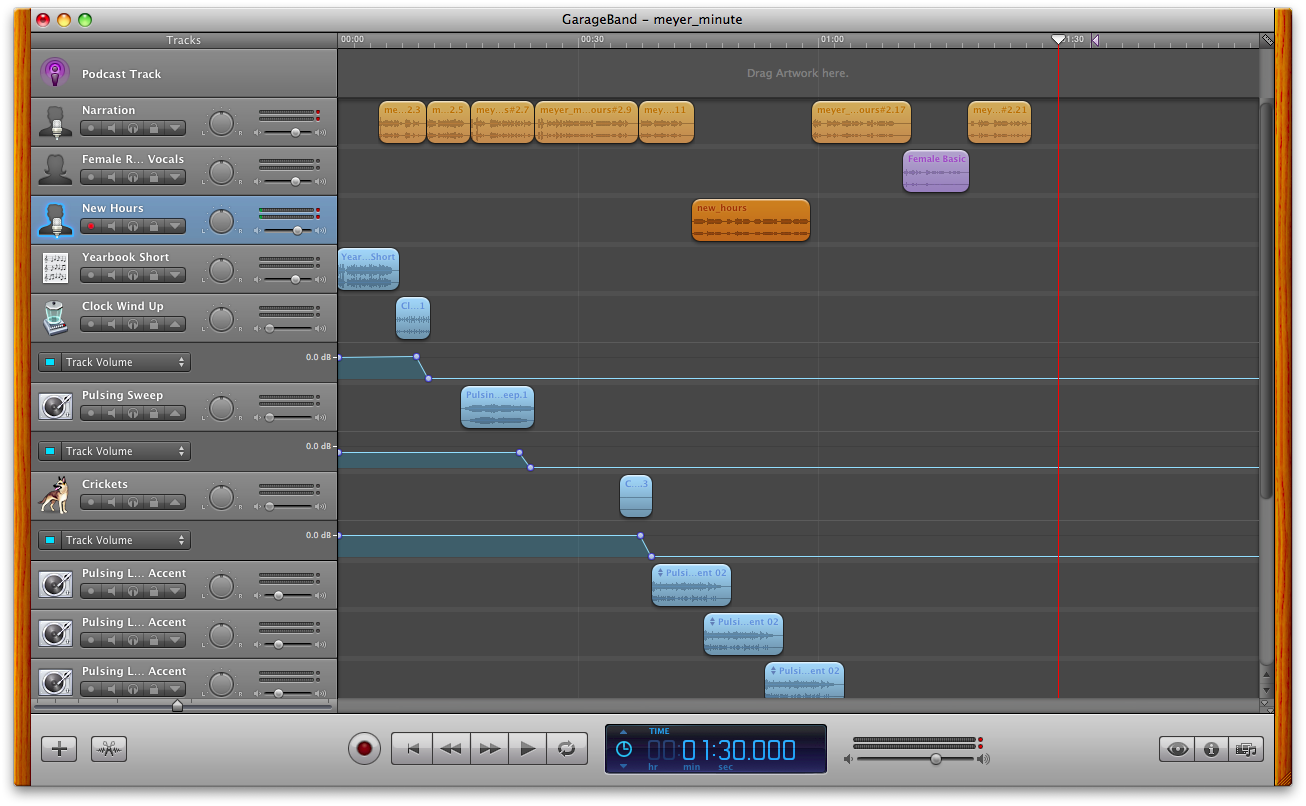
\includegraphics[width=0.75\textwidth]{img/MusicEditor.png}
   \caption{Example of music splicing software. Relevant is the time-sequence manipulation with blocks.}
   \label{img:MusicEditor}
\end{figure}


\subsection{Sketches, other examples}

\section{Cubli Behavior}

The purpose of this project was to add new behavior to Cubli, without removing any. That is, one of the main goals was to preserve all existing functionality.

As such, it is necessary to create a state for cubli in which it performs choreographies. This is distinct from another, "standard" state, in which cubli behaves as it previously did.

The former, called "choreography" state, should be entered at the start of the performance and exited at the end.

\subsection{Choreography State}

In the choreography state, a cubli should keep track of the elapsed choreography time, and execute the action corresponding to the current time.

\section{Communication}

It is straightforward that communication between cubli and choreographer is necessary in order to put choreographies into action. However, the exact implementation of these communications is not, itself, obvious.\\

The observed particularities of this mode of UART transmission are described as follows:
\begin{itemize}
\item communications involve the transmission of 8-bit "packets" ( or "characters" ) in sequence
\item all devices share the same frequency channel. i.e, when a device sends a packet all other devices immediately receive it
\item the packets themselves are not signed or identified
\item there is a significant probability of a cubli failing to receive a packet, or receiving packets in the wrong order
\item there is a much lower probability of the computer failing to receive a packet
\end{itemize}

Identification, verification, and disambiguation of messages, if necessary, have to be implemented within these constraints.\\

Identification: In a scenario where only one cubli and computer communicate, it would be possible to forego the encoding of sender and recipient inside messages, as they are implied in one-on-one conversation. However, since the goal of this project is to have a choreographer functioning with several cublis simultaneously it becomes necessary for communications to explicit the devices from which they are emitted and to which they are intended.\\

There would be several ways to implement this, notably at the packet level - for example, using some bits from each packet to encode the sender - or at the message level - each group of chunks containing a header with the relevant information.\\

The principal advantage of the first method is that it enables the removal of transmission failures in the case of simultaneous emission, as it allows identification of packets in any situation. In simpler terms, for example if two packet sequences are sent simultaneously by two devices: the orginal sequences can still be disambiguated by organizing packets based on the senders - which are encrypted in every byte - and the garbled messages can thus be reassembled.

However, it also means that the more devices a protocol accepts, the lower the amount of information available in each packet for data itself. For example, if a maximum of 10 devices can be connected at once, 3 bits of every byte must now be dedicated to identification metadata, which leaves 5 bits for data: instead of 255 possible values p. packet, we now have 32. This is disadvantageous as the amount of "wasted" space increases significantly with message size when using this method.\\

\begin{figure}[ht]
   \centering
   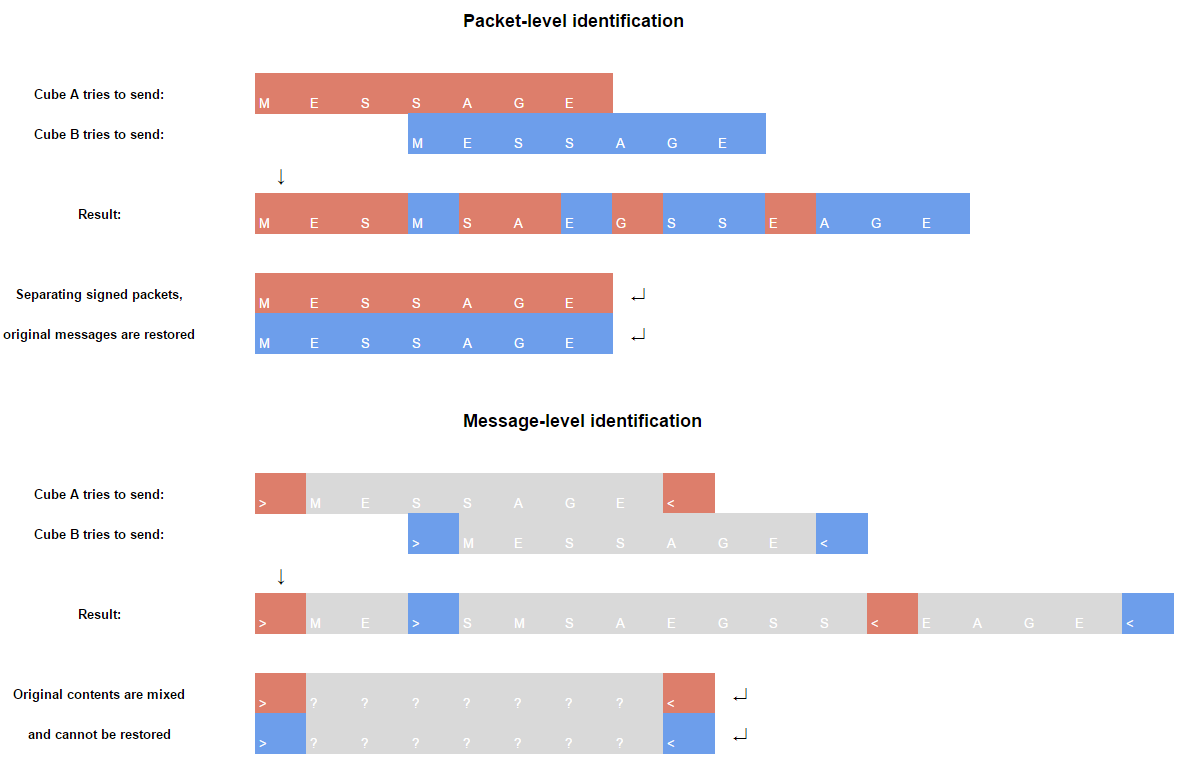
\includegraphics[width=0.75\textwidth]{img/disambiguation.png}
   \caption{Recovering mixed-together messages with packet-level or message-level sender identification.}
   \label{img:disambiguation}
\end{figure}

It follows that the second method is preferable where the risk of simultaneous message emission is relatively low. We see later that this is indeed the case. \\


Verification: Does this project require that the integrity of messages be verified? For any scenario where the rate of successful transmission can be expected to be lower that 100\%, ensuring that messages are emitted and received as intended is essential. In addition, though it requires extra effort during development, the necessary overhead to verify message contents during operation is low enough that it would be reasonable to implement it here even if a \~100\% transfer rate was expected.




\section{Failure Scenarios \& Responses}
This section discusses the planning of failure estimation and handling.
\textit{What could go wrong, and what cubli should do if it does}.\\

As in every complex system, there are certain and uncertain likelihoods of something going wrong at any stage and for a multitude of reasons.\\

In this section we attempt to identify the most important failures which can affect any step of choreography, and come up with appropriate responses. These responses shape the entire project execution in no small way.\\

Here, failure importance is considered in the risk-analysis sense. That is, it is based on two factors: probability of occurrence, and severity of the disruption. Disruption is the amount of deviation from expected behavior, weighed by subjective preference for avoiding the resulting erroneous behavior. \\

Regarding the usefulness of this section:\\

Of the two factors taken into account above, the second, that is the disruptions themselves, can in many cases be deduced logically ( "if A fails, then B fails. If both fail, X will not be fulfilled" ), though it generally still contains probabilistic unknowns. The first factor, probability of occurrence, has to be at first intuitively gauged, since at the outset very little is known about hardware and software reliabilities, and only later measured.\\

For this reason, failures can at the start be incorrectly evaluated, their consequences or the responses misunderstood, or even simply not expected. As the project progresses, the actual importance of failures - through both factors - becomes gradually clearer.  This evolution leads to modification of the planned implementation in order to account for these corrections.

\subsection{Choreography Failures}

Cubli's ability to learn and perform movements is impressive and works very well. It still happens that moves fail with varying likelihoods - especially difficult moves. This is the principal source of failure in a choreography.

As such, the strategy for recovering from failed moves is important, and though in any case the perfect execution of the choreography is lost when such a failure happens, different recovery methods work to salvage different aspects of the remaining choreography execution.

A few examples of potential recovery methods and their consequences:\\

\begin{description}
\item[A.] Letting unaffected cubes continue their program, without waiting. The affected cube recovers as fast as possible, and then continues its program with a delay with respect to the others.
The particularities of this strategy are as follows:

\begin{itemize}
\item[-] Sync between timelines is not preserved in case of failures
\item[+] Non-failed cubes' timelines remain true to their intended versions.
\item[+] Almost no intervention is required, and the communication cost, as well as likelihood of aggravating a failure are low.
\end{itemize}

\item[B.] Notifying all cubes in case of failure, pausing all devices until the issue is resolved, and then resuming all the choreography all at once.

\begin{itemize}
\item[-] The more procedures are put in place to ensure the correct behavior of all cubes, and the exactitude of sync, the more complex this strategy, and the longer it takes before choreographies resume. 
\item[+] If done correctly, the simultaneity of all timelines is preserved, and only the length of the global choreography is increased by a failure.
\end{itemize}

\end{description}
\cleardoublepage
\chapter{Implementation}\label{sec:implementation}

This section goes over the solutions and implementation that were selected over the course of the semester project. \\

To ensure clarity, this part will be keeping with the three-module  structure established in the previous chapter. 

\section{User Experience - The Choreographer App}

\begin{figure}[ht]
   \centering
   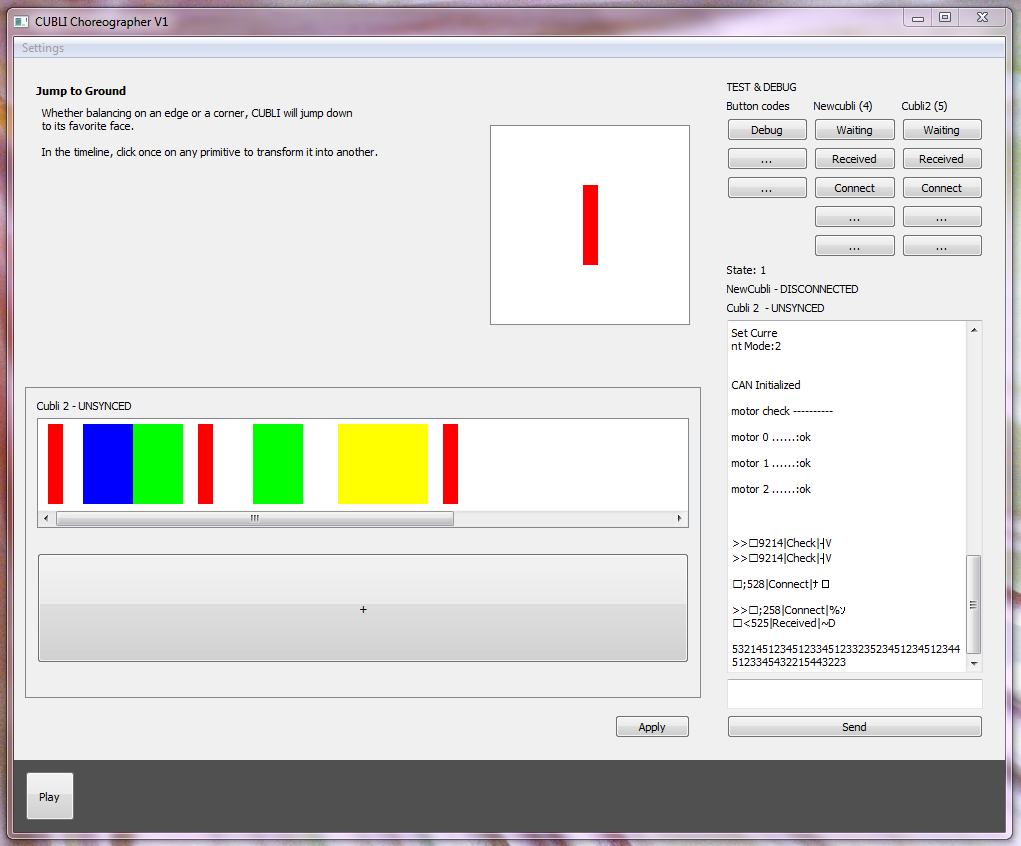
\includegraphics[width=0.75\textwidth]{img/ChoreographerGUI.png}
   \caption{The CUBLI Choreographer Graphical User Interface.}
   \label{img:ChoreographerGUI}
\end{figure}

In the end the choreographer application is quite close to the initial concept. Whereas one could have expected it to evolve differently, the first approach has remained a valid implementation during the project and thus the concept has not deviated much from the outset.\\

One notable addition is the creation of a debugging panel, to the right of the main window, which can also be completely deactivated and hidden. When it is visible however, it provides access to all the communications, and to manually send out messages from the computer, or to simulate incoming messages from cubes.\\

\begin{figure}[ht]
   \centering
   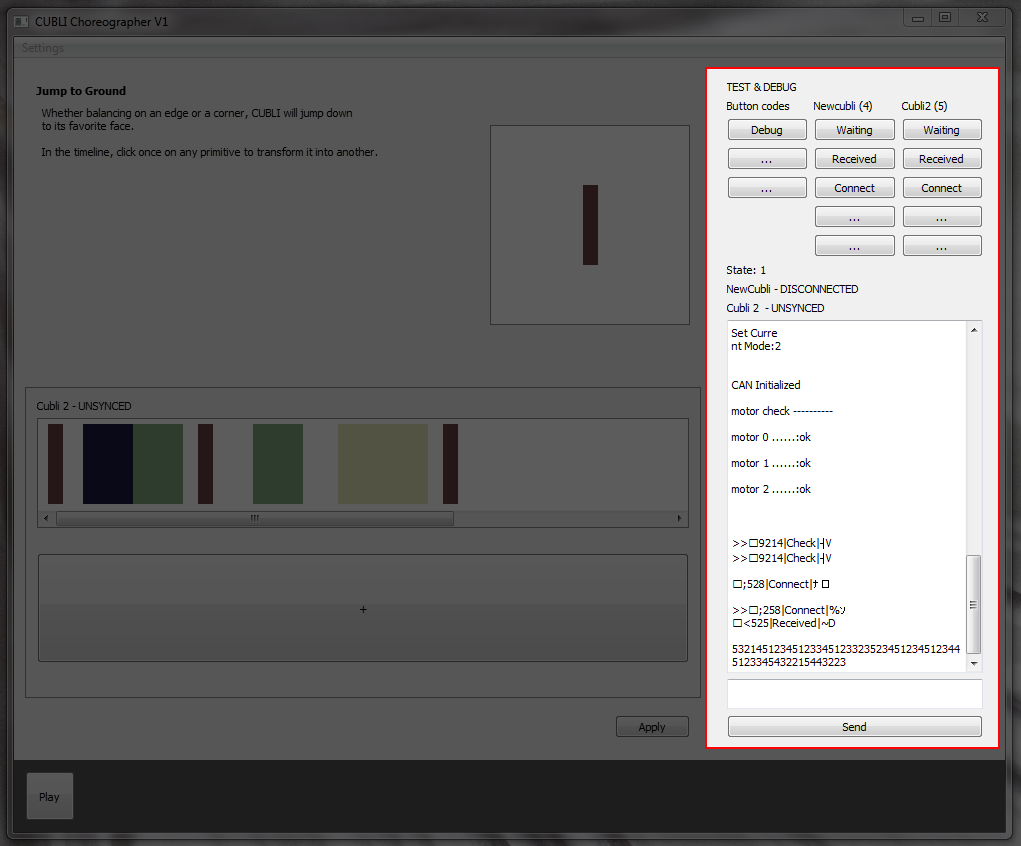
\includegraphics[width=0.75\textwidth]{img/DebugPanel.png}
   \caption{The debugging \& information panel.}
   \label{img:DebugPanel}
\end{figure}

\subsection{Language}

C++ was the obvious choice for a language for three reasons: i) it allowed to reuse code structure from the C source with few modifications ii) the communication protocol could be compiled on the two different machines from the same C file, thus greatly reducing the chances of bugs appearing due to unvoluntary divergences in the protocol source code iii) On the first targeted machine, it had readily available libraries for all the necessary peripherals and UI elements, as well as useful object-oriented features. 
The libraries in question were taken from the QT development kit, a decision which was not obvious as the advantages of QT over Visual Studio appear marginal. \\

Just as the final application, in debugging mode, has two main panels - one concerning the user interaction, specifically the creation of timelines and control of the choreography evolution; one displaying communications through the serial port and state machine information - the development process was centered around two features : i) serial port communication and ii) timeline creation, transfer, and execution. 

\subsection{App Components}

Here we clarify the contents of various parts of the choreographer app source, as available in the Github repository. For each part, a general explanation is given, and if any are relevant, is followed by more technical details.

\subsubsection{Main Window}

First and foremost, this class displays and sets up the main viewport. It defines the action for all the buttons, and provides functions for updating text fields such as the app information.

As such it is mostly QT-specific code, with several functions handling the app behavior when connecting or syncing with cubes.

\subsubsection{Serial Manager}

Serial port communication was the first implemented functionality of the app, relatively easy to write thanks to the already well-built QT serial port libraries. In detail, successful sending entails: 

\begin{itemize}
\item setting the port name ( Later, a panel for setting those options easily, which among other things contains a drop down list enumerating the available port names was added ) 
\item setting the serial parameters, such as baud rate, hardware flow control and so on to the same values as inside cubli ( Baud rate of 115200, ) 
\item open the port. This is straightforward through a simple function call 
\item send bytes through the port. A function call is all that is needed here as well. 
\end{itemize}

Receiving is handled in an interrupt, which hands over control to a function written for that purpose.\\

Among other things this function displays all the received bytes in a serial stream display panel. In addition, any bytes sent by the Application over serial are also displayed in the same serial stream display panel with a line prefix of '>>' \\

The class named Serial Manager was created in order to handle those actions. 

\subsubsection{Timeline}

Created and displayed when each cube connects to the application, a white rectangular canvas on which the user can place, modify or remove color coded squares is meant to represent the chorography - the horizontal axis representing time, - and, as such, is called a Timeline. Each square, called a Primitive, represents a specific action of cubli, and thus, one or several Timelines, each containing a sequence of primitives, together represent a choreography. \\

\begin{figure}[ht]
   \centering
   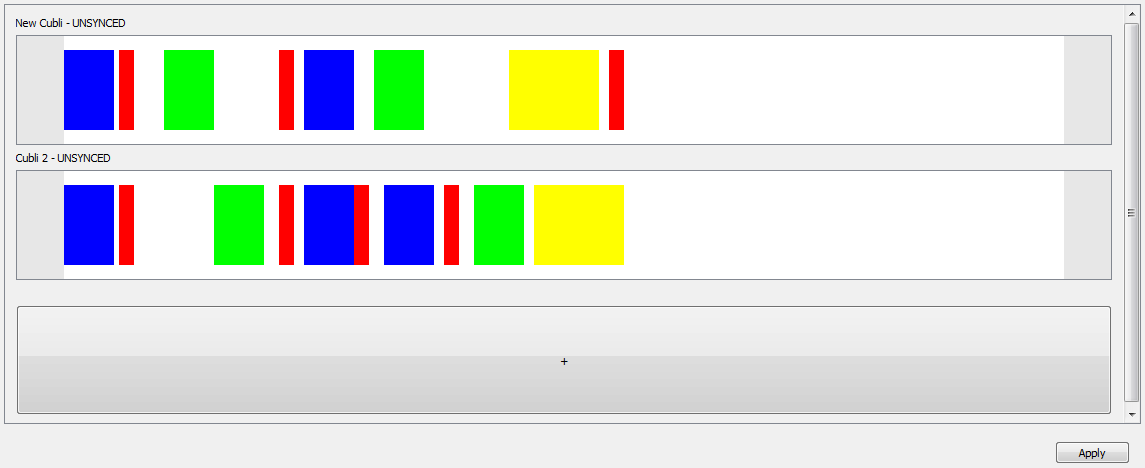
\includegraphics[width=0.75\textwidth]{img/TimelinesPanel.png}
   \caption{The Timeline Editor panel.}
   \label{img:TimelinesPanel}
\end{figure}

For this purpose, within this projet the timeline canvas, or "Graphics Scene" in QT nomenclature, was programmed to respond to user interactions in the following ways: 
\begin{itemize}
\item Clicking on empty space creates a new primitive at that position 
\item Clicking a primitive modifies it, cycling through the available types one at a time 
\item Double clicks are no different from two simple clicks 
\item Left click-and-dragging a primitive moves it based on mouse position 
\item Right clicking a primitive erases it 
\item Right click-and-dragging erases all primitives under the cursors path 
\item Left click and dragging on empty space has no effect 
\end{itemize}

\subsubsection{Timeline - Technical Addendum}

Programmatically this behavior was encoded as follows: 

\begin{itemize}
\item When the left mouse button is pressed within the timeline bounds, the application checks whether a primitive is present under the cursor. Depending on whether that is the case, different actions are assigned to mouse events immediately following this one. Furthermore, the primitive present under the cursor, if any, is selected for later handling 
\item ...
\end{itemize}


\subsubsection{Primitive}

The primitive class is an extension of simple rectangle objects in the timeline, adding extra properties such as type, and automatically assigning styles, width, or positions, thus making them simpler to display and move around. These extended rectangle objects are meant to visually represent the action primitives of a cube in the choreography.\\

This class provides methods for easily accessing certain properties, modifying, or moving the primitives around, for example without running into each other.

\subsubsection{ComStateManager}

 The ComStateManager class is the part of the application which handles communication responses, i.e. \textit{what to send and when}.
 
Any message sent to the cube from the app means a call to this class. It is also where cube statuses are stored, which allow it and other parts of the application to take into account whether particular cubes are connected or not, syncing or not, and so on.\\

Which message must be sent is necessarily determined in this class' logic.
It accomplishes this through a state machine, that has a corresponding response for every incoming message or application call.

\subsubsection{SettingsDialog}

SettingsDialog is responsible for putting together the settings dialog which appears when the serial port settings are to be modified, and storing their values.

\subsubsection{Main.cpp}

Main runs the mainwindow code, launching the app, and any necessary QT routines.

\section{Communications}

The source for the message protocol fits inside one cpp file and accompanying header. It mainly creates or deconstructs strings or characters, in order to transmit and receive messages which satisfy the required specifications.\\

Of course, the concept of communication protocol as a whole pertains to more than uniquely this message-transmission code. It also englobes the determination of how the machines ought to behave when contacting each other, which in practice is encoded all over their code ( see communication state machines, MainWindow, etc ). However for the sake of consistency the particulars of these protocols are discussed here.\\

One of the difficulties during this project was the unreliability of the UART behavior in the cubli microcontroller. Thankfully the communication protocol was designed to be quite robust from the get-go, which seemed at the time like a potentially unnecessary amount of safety, though it proved essential.

\begin{figure}[ht]
   \centering
   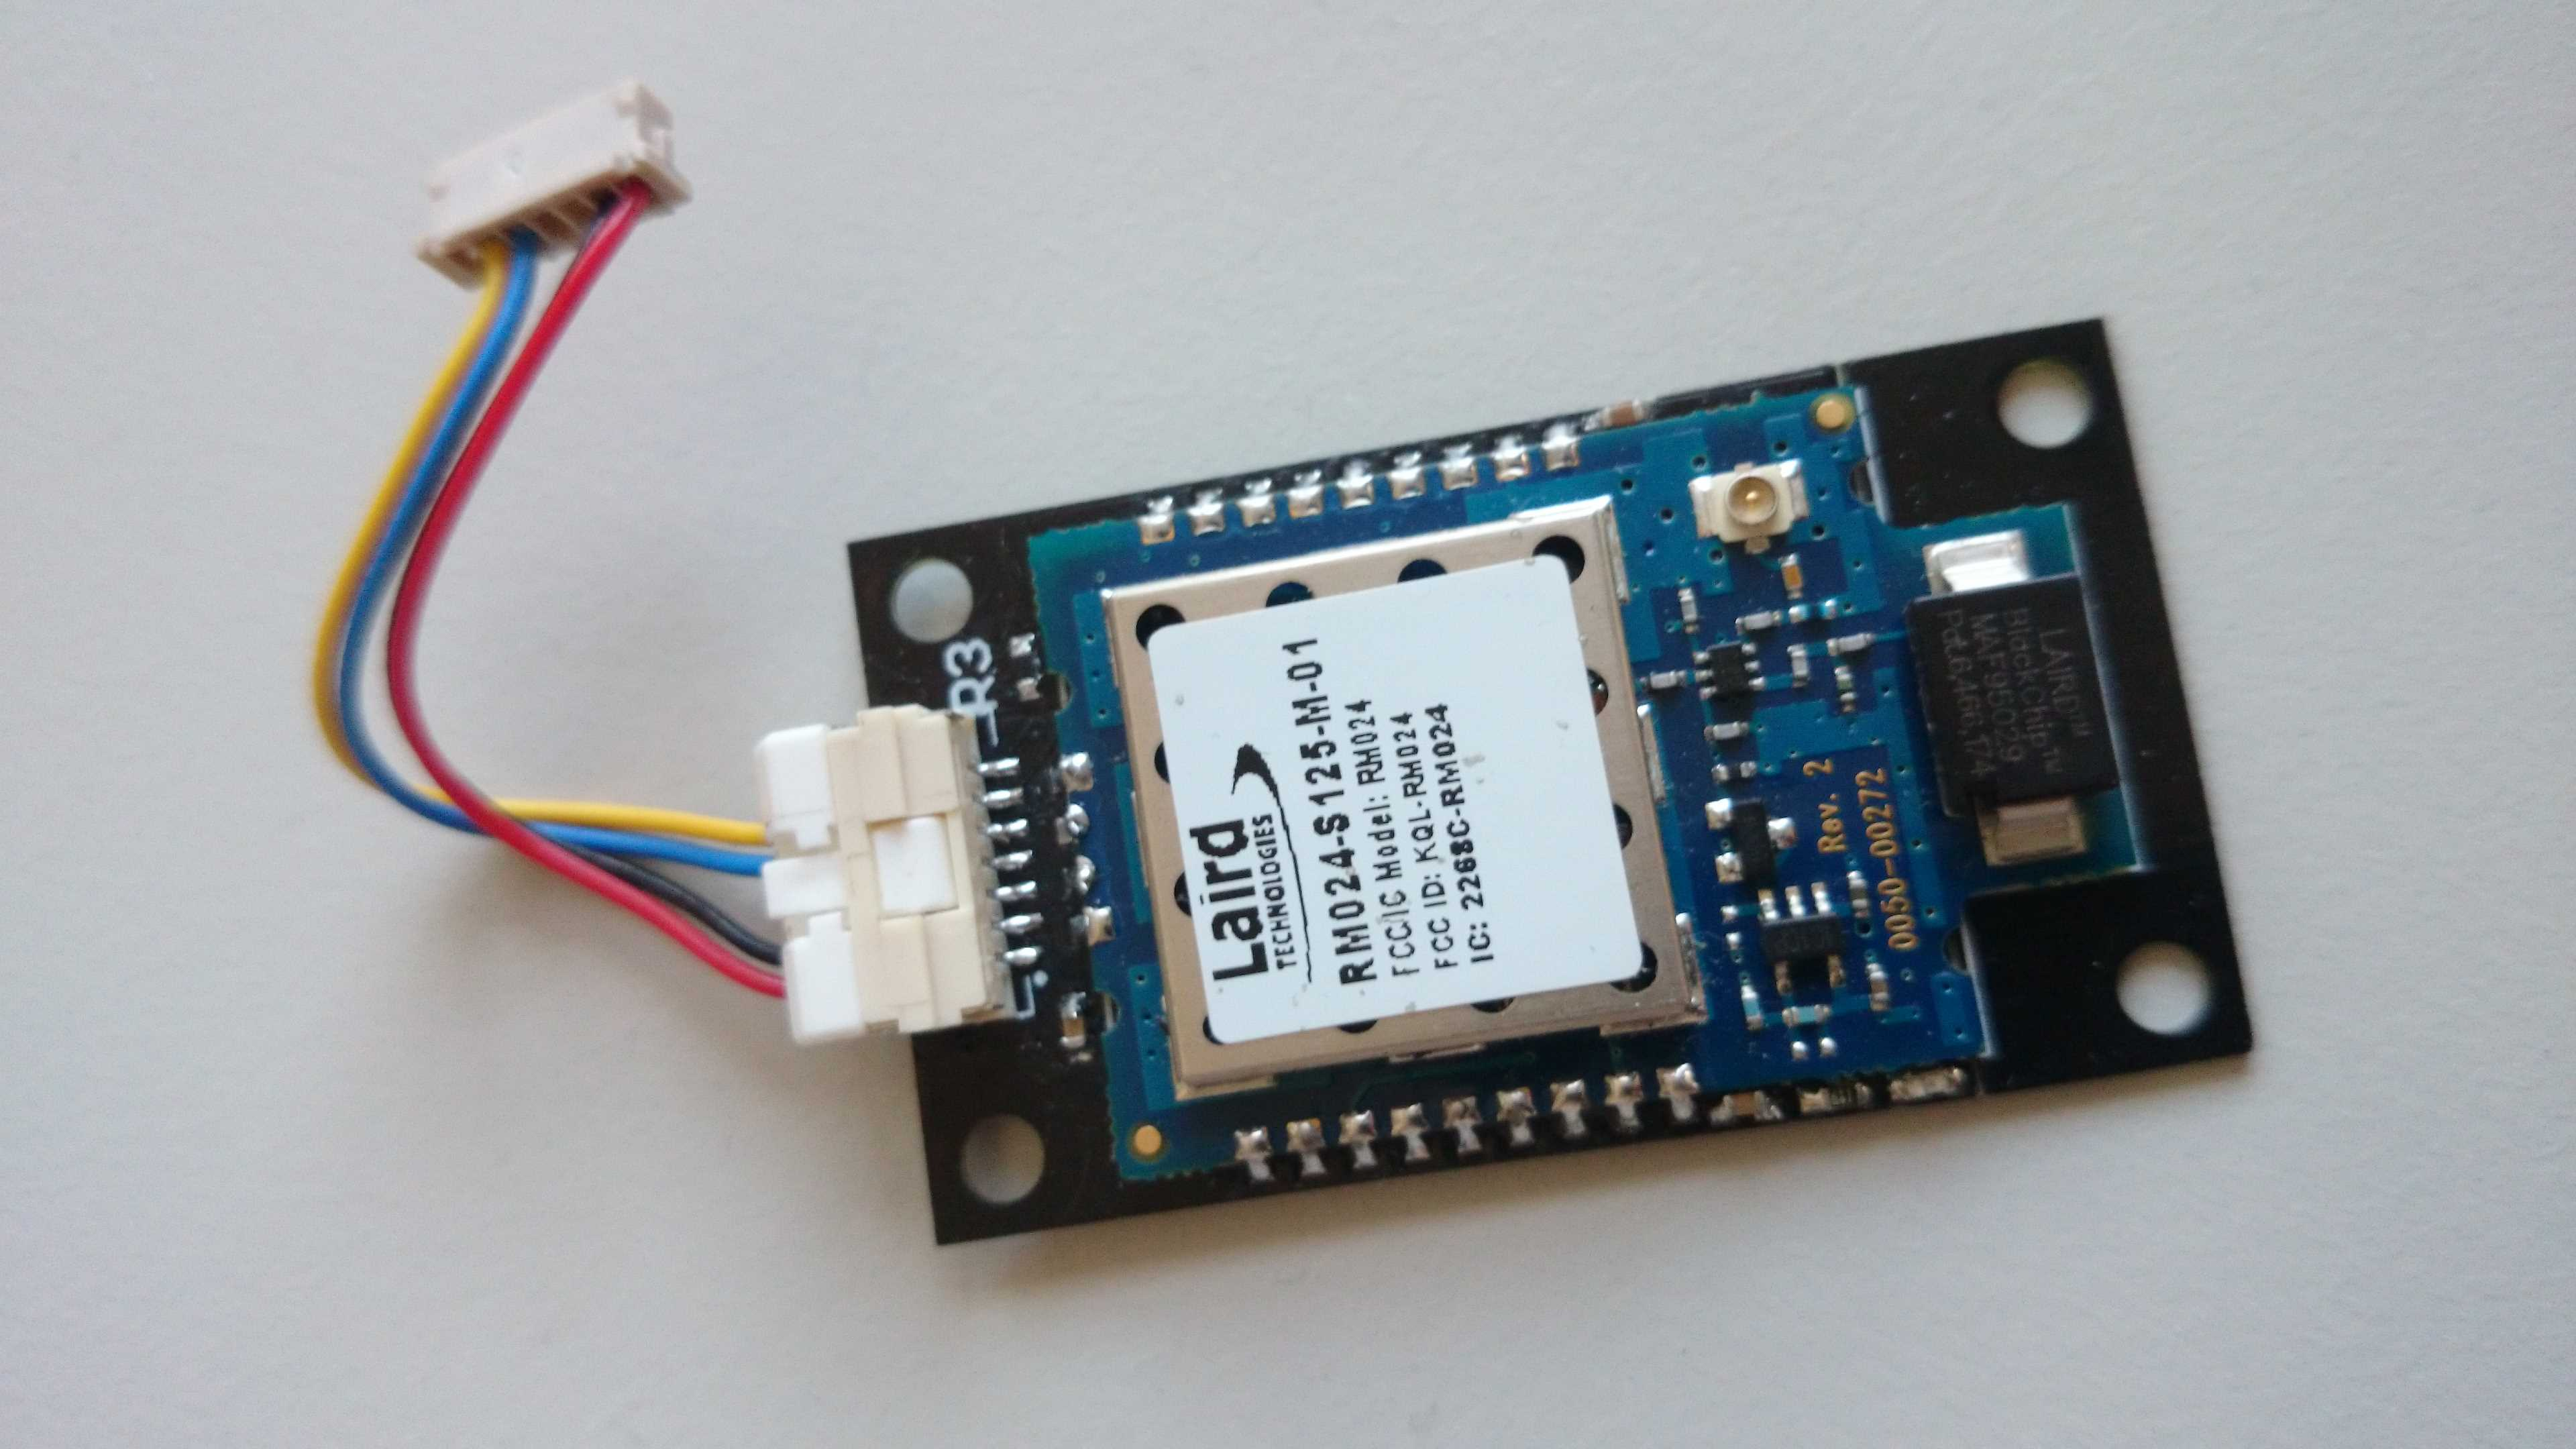
\includegraphics[width=0.75\textwidth]{img/LAIRD-radio.jpg}
   \caption{Radio used in the Cubli hardware.}
   \label{img:LAIRD-radio}
\end{figure}

The inability to work with the assumption that 'the majority of messages would be able get through successfully' also meant that communication protocols were not simply a formality, and had to be designed with contingencies in mind. This made this module an interesting, though larger than anticipated, part of the project.

\subsection{com\_protocol}

Principally, this code transforms a message's code, additional content, and metadata into a normalized string of characters which can be sent one byte at a time over UART. And vice-versa.\\

The message \\

[Message deconstruction] \\


\subsubsection{Header}

The header, com\_protocol.h contains enumerations for all the message codes, communications states, and a few other which are shared between cubli and computer, as well as some macro expansions which concern communication settings.\\

[Message code table]\\

It also contains two compile flags:\\

\begin{itemize}
\item[] COM\_VERBOSE

	if this flag is defined, messages also contain a human-readable appendix expliciting the relevant message code, and extra content.\\

\item[] COM\_DEBUG

	if this flag is defined, extra information pertaining to failure when decrypting messages is displayed as plain text. This is for example useful when messages are not getting decrypted though they are transmitted correctly.
    
\end{itemize}

\subsection{Protocols}

\subsubsection{When Syncing}
\subsubsection{When Connecting}
\subsubsection{When ...}

\section{Cubli}

In order to avoid introducing new bugs, care was taken to build on top of already-existing functionality rather than to modify it, as much as possible.

This means that except for a few additional line of codes, the controllers remain unchanged, and the code relevant to this project is composed of additional tasks for communication, choreography, and additions in mode management.\\

These relevant parts are what will be discussed here, rather than the entire cubli source code.

\subsection{Affected Tasks}

The main routines executed inside cubli softwares are managed by a realtime OS, which compartimentalizes them into various tasks, giving to each their respective processor access time, depending on their priority, period, and so on. This allows several processes to run in parallel, without necessarily affecting each other.

As an example, some tasks inside cubli are responsible for regularly checking that user inputs have been made, while others are responsible for the high-frequency control necessary during movements, such as the LQR controller task for balancing.

This subsection describes the code modifications and additions in this project, to the relevant tasks

\subsubsection{ModeManagement Task}

Originally a task responsible for updating the global variables responsible for deciding which controllers get activated based on the current mode ( which is originally incremented through the press of a respective hardware button ), it keeps its functionality in this project.\\

New modes are created for choreography, corresponding to the movement primitives, while the original modes are renamed to button modes, and relevant code sections are modified to make the new and original modes cohabitate. To this end, the original and old modes are distinguishable, allowing behavior which was only needed in old modes to be disabled for the new modes only.\\

[Old modes and New Modes]\\

[Pause upon resetting cubli on face?]\\

\subsubsection{ComManagement Task}

This task contains both the code responsible for reading from the UART buffer, and a state communication machine similar to the one in the choreography app.\\

One notable difference between the communication behavior of cubli compared to the app is that its communication state machine is triggered regularly rather than on specific event occurences.

\subsubsection{ChoreographyManagement Task}

The choreography management task is only active during choreography, in which case it keeps track of the current primitive and run time, and adjusts the mode accordingly. It also implements behavior for pausing the choreography and notifying other cubes through the communication management when a move fails.

\subsubsection{TimelineStatus Task}

This code is responsible for storing the timeline information.\\

A cube stores only one timeline, its current timeline, which it does not modify. Alongside it, is a 'cache', a temporary timeline which is filled during sync, and then copied to the current timeline if the sync was successful, or discarded if unsuccessful.\\

[Limits of timeline storage, etc]

\subsubsection{Controller Tasks}
Some controller tasks were modified, to the smallest necessary extent, to fit with the choreographer functionality. Care was taken to ensure that the controller behavior would remain unchanged outside of choreography (i.e. with the relevant code sections being bypassed by if-clauses checking for choreography activity)

Three functionalities had to be added in the controllers' code:
\begin{itemize}
\item the ability for cubli to fall down to a face on its own
\item regulating the braking time to help synchronize choreographies
\item notifying the choreography management task when primitives are successful
\end{itemize}



    




\cleardoublepage
\chapter{Using the Choreographer}\label{sec:usingthe}

This section is a short user manual for the Choreographer project.
Step by step, the actions to be undertaken in order to create and execute a choreography are detailed.\\

In this chapter it is assumed that the following are available:
\begin{itemize}
\item A computer running the Windows ( 7 or above ) operating system.
\item A functional wireless serial port device connected.
\item One or more Cubli robots with the choreography firmware flashed.
\end{itemize}

\section{Preparation: Testing and Training Cubli}

This is an \textit{optional} step, which consists in:

\begin{itemize}
\item[] Turning Cubli on, and checking that the batteries are full
\item[] Through the mode button, having Cubli perform all the basic moves on the proper surface until it has mastered them.
\end{itemize}

Taking these precautions results in smoother choreographies, and ensures that the Cubli robot is functional.

\section{Connecting to Cubli}

First, launch the choreographer app, available as an executable in the github repository.

Once the app is launched, a serial port selection and settings dialog pops up ( \textit{c.f. Figure \ref{img:SerialSettings}} ). Select the appropriate serial port. It must correspond to a wireless serial device connected to the pc.

\begin{figure}[ht]
   \centering
   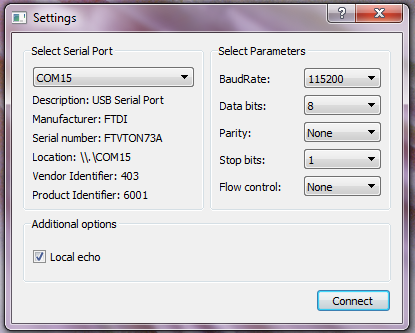
\includegraphics[width=0.75\textwidth]{img/SerialSettings.png}
   \caption{Settings Window for the serial port, displaying an example of correct values.}
   \label{img:SerialSettings}
\end{figure}

\textbf{Note:} If closed, the settings dialog remains available through the menu bar of the main window.\\

At this point, turning on a Cubli will automatically connect it to the application and its timeline should appear. You can also manually attempt to connect to Cublis which are powered on, by pressing the large '+' button in the middle of the main window.


\section{Make Your Own Choreography}

Once a cube's timeline is visible, it is possible to create or modify the choreography by using the mouse buttons within its bounds - that is, the white area.\\

On an empty part of the timeline, left-click once to create a primitive.

Left-click that primitive again to change its type.

Click-and-drag the primitive to modify the timing.

Right-click any primitive to delete it.\\

Information concerning the last-clicked primitive is visible in the top panel of the main window.\\

\textbf{Note:} when moving a primitive, it follows your mouse unless there isn't any space for it.\\

When cycling through primitive types, due to the change of length, it is possible that a primitive no longer fits between the ones surrounding it. In this case all the following primitives are displaced to make space.\\

Interact with the various timelines until you are satisfied with the choreography.


\section{Sync Your Choreography to the Cubes}

Press the apply button and wait for the app status to show "Sync Successful".\\

\textbf{Note:} It sometimes occurs that a cube does not respond too long while syncing, in which case the sync is cancelled by the application, and that cube is disconnected. In that case, ensure that the cube is turned on and functional before trying again.\\

Once the sync is successful, all connected cubes have the choreography stored in the exact state it was when the apply button was pressed. 
At this point further modifications to the timelines in the app will not be synced until the apply button is pressed again.\\

\textbf{Note:} Timelines are not deleted from the editor panel when a cube is disconnected, in order to prevent accidentally deleting choreography data. As such, they remain visible, but will not be synced until the cube is reconnected. Reconnecting to a cube is the same process as in the '\textit{Connecting to Cubli}' step above.\\

\textbf{Note:} In addition, when Cubli is turned off, all timeline information is cleared from its memory. As a result, it is necessary to once again sync any cube that has been restarted.




\section{Run the Choreography}

Once a timeline is stored in the cube, it is ready to execute the choreography. 

In order to do so press the "Play" button.\\

This will initiate a countdown to the start of the choreography, during which all cubes must confirm that they are performing. If one cube or more do not provide confirmation the choreography is cancelled and must be attempted again. The non-responsive cube is automatically marked as disconnected.\\

It is also possible to manually cancel the countdown by pressing the "Play" button, which is at this point displaying the countdown value.\\

After the countdown the choreography is started, and cubes will attempt to complete their current primitive even if they fail. No user interaction with the app is necessary, however in the event that they fall on an unrecoverable face, Cublis must manually be reset back to their main face.

\begin{figure}[ht]
   \centering
   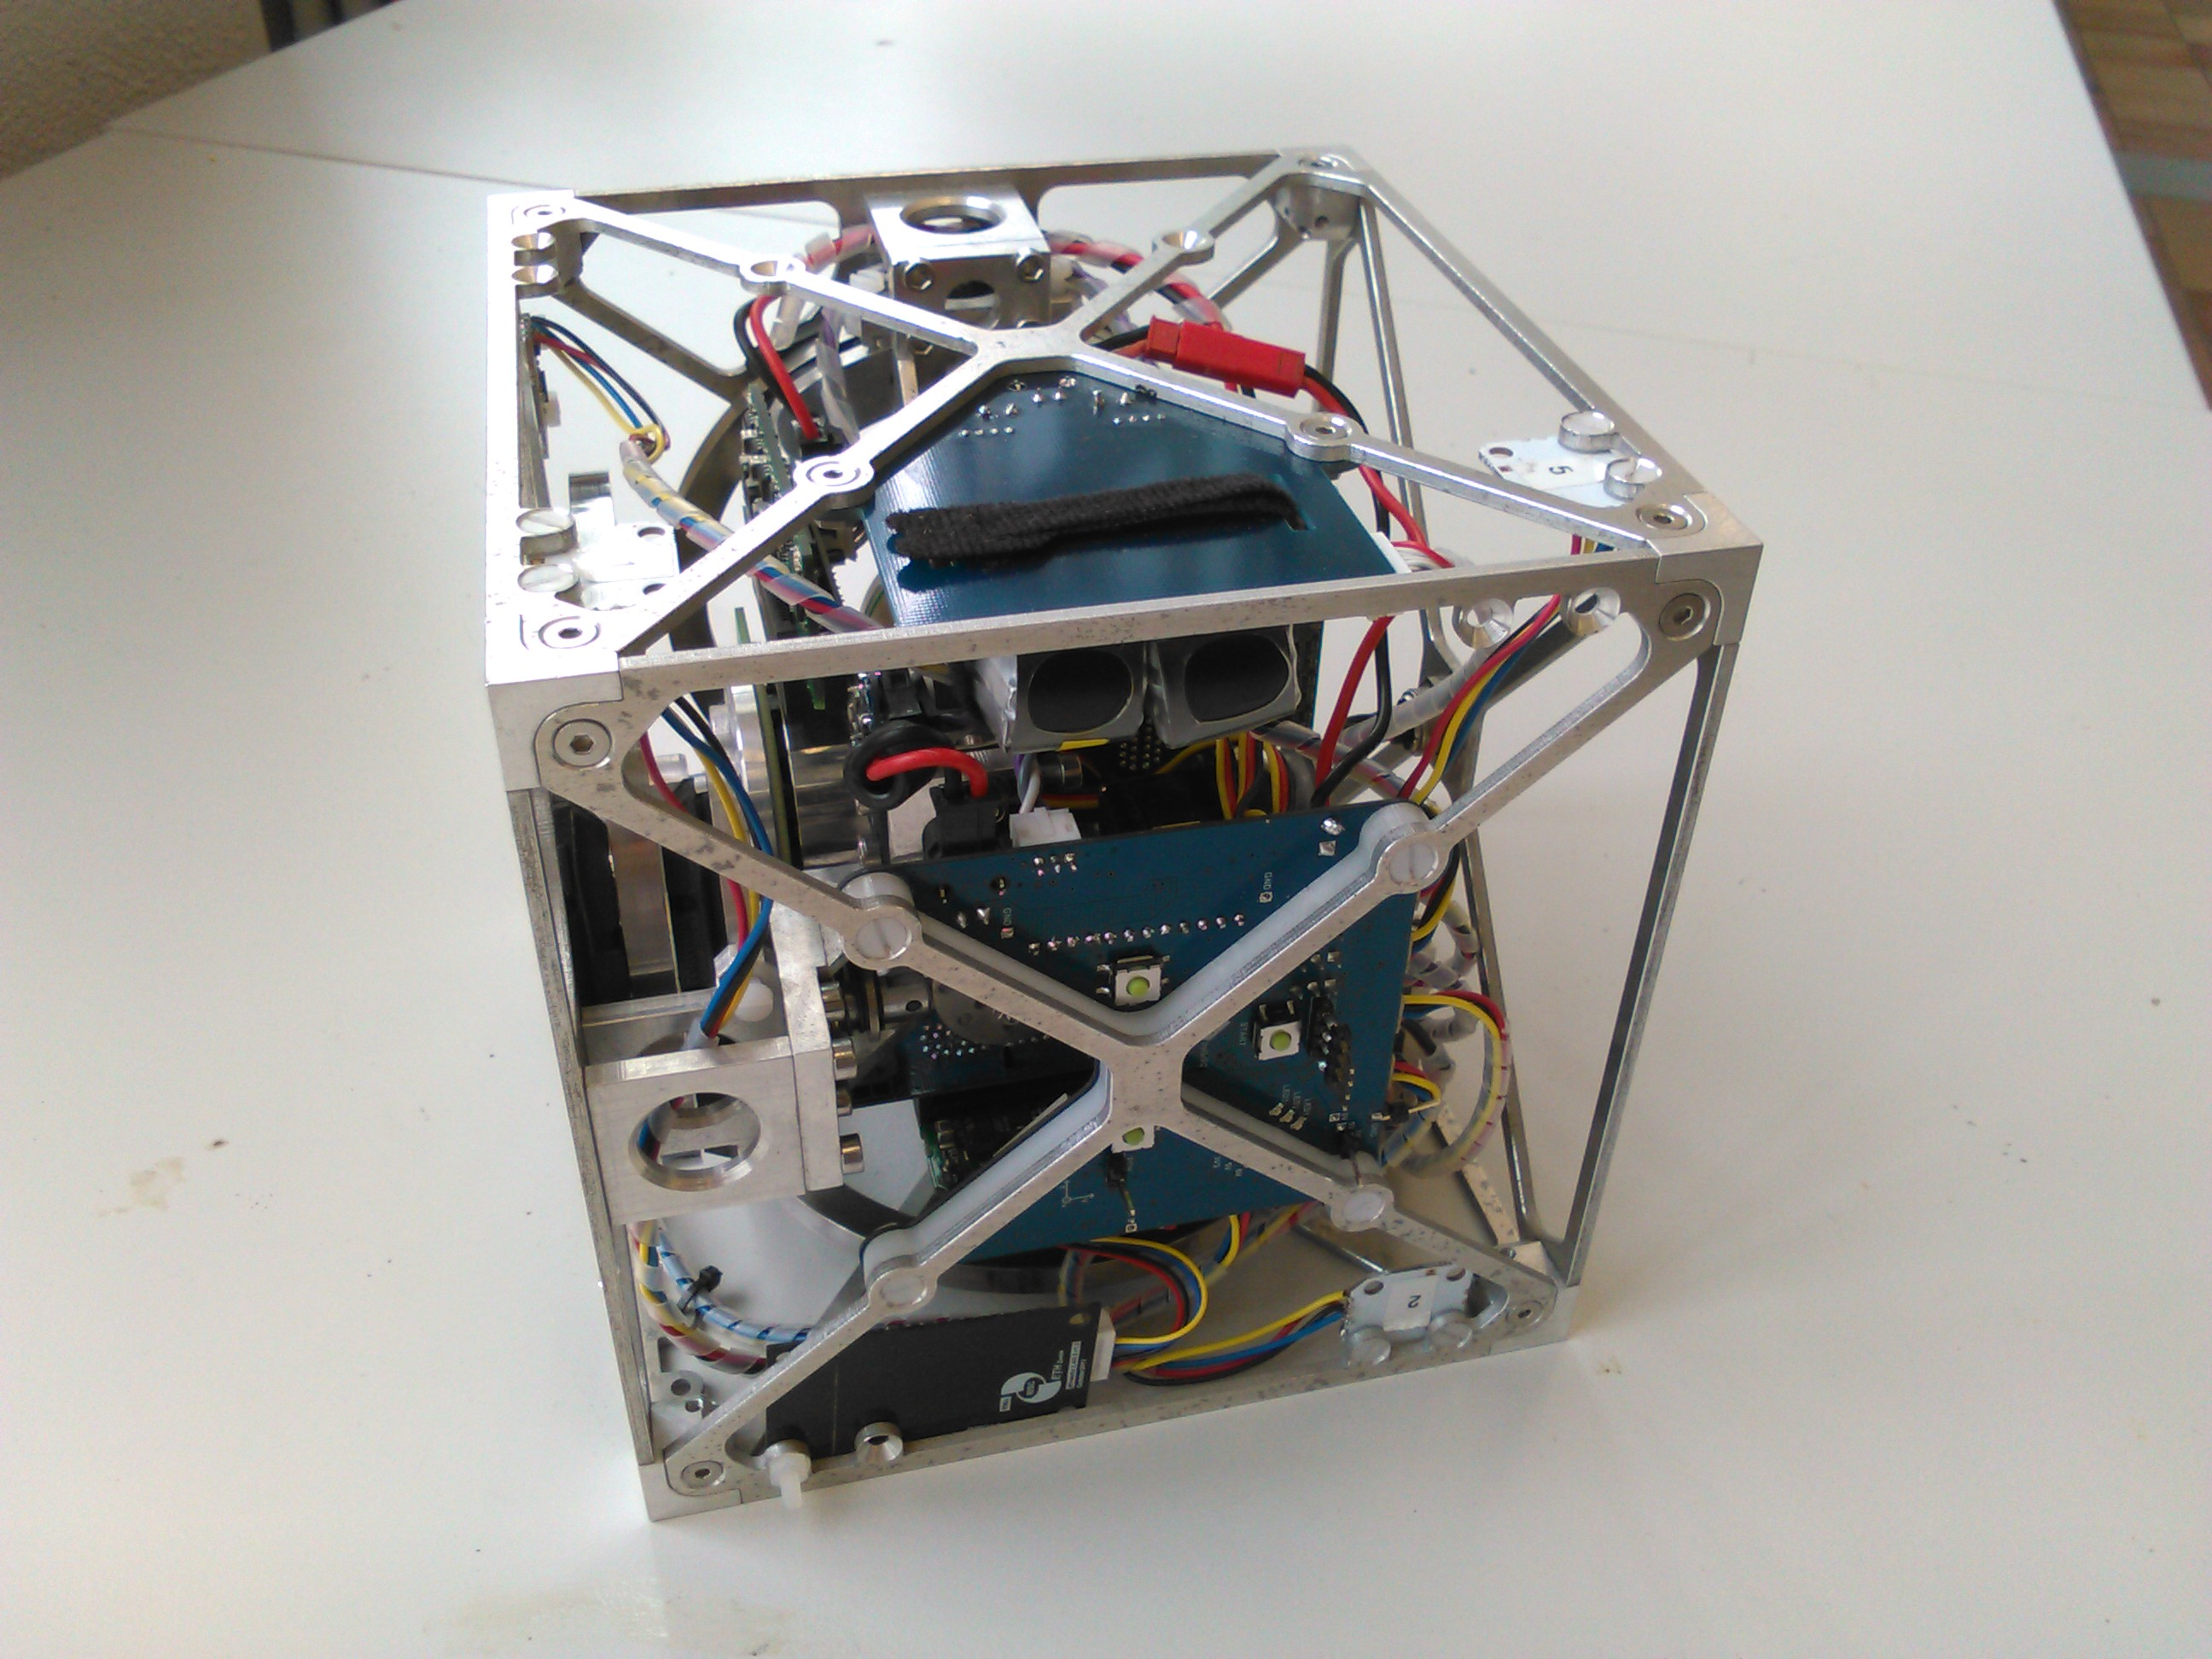
\includegraphics[width=0.75\textwidth]{img/MainFace.jpg}
   \caption{Cubli set-up on its main face. Note the orientation of the buttons on the front-facing panel.}
   \label{img:MainFace}
\end{figure}


\section{Stop the Choreography}

The choreography stops automatically when it reaches its natural end, that is when all cubes have completed their last primitive. \\

It is also possible to stop it manually, by pressing the "Stop" button, which can be seen in place of the "Play" button in the UI once the choreography is running.


\cleardoublepage
\chapter{Results \& Discussion}\label{sec:results}

\section{Communication Results}

\subsection{Message Transmission}

Running tests to quantify the quality of communications between Cublis and Computer, we obtain the data in Figure \ref{img:comStats}. Specifically, these numbers where obtained through testing of the sync protocol.

\begin{figure}[H]
   \centering
   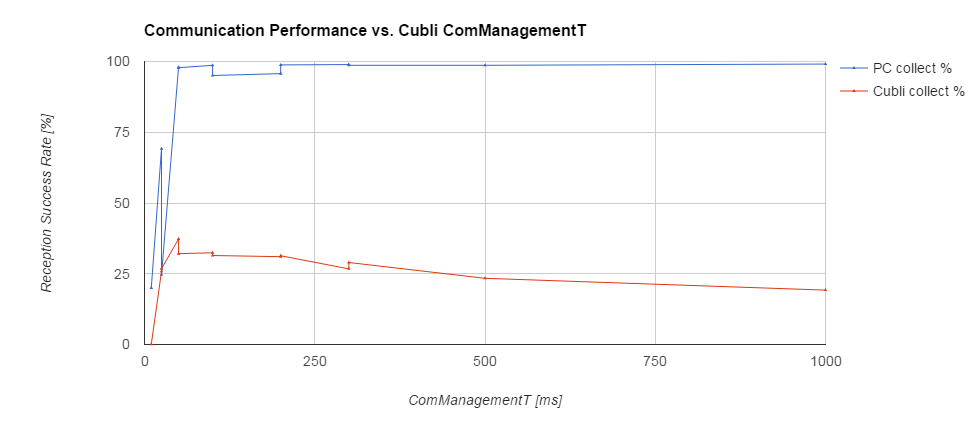
\includegraphics[width=1\textwidth]{img/comStats.png}
   \caption{A measure of the average communications success rate, with varying communication-update periods in Cubli.}
   \label{img:comStats}
\end{figure}

As such we observe that on average, there is a 30\% chance of Cubli collecting a message. This further means that if we are to send Cubli the same message 5 times, the probability of at least one message being successfully received is 85\% and for 10 identical messages, the same probability becomes 97\% .\\

In addition, measurements were ran at 50 ms ComManagementT sampling time, replacing the wireless adapter with a direct wired connection to the PC. Over a large amount of messages, the resulting success rate for reception in Cubli increased to 50\%. It is therefore hypothesized that the remaining 50\% of losses originate from inside the software, particularly the way that UART reception is handled.\\

Running similar test during other protocols yields similar results, with Cubli's reception rate rarely exceeding 40\%.\\

Finally, through all the tests , and the whole project, messages from two Cublis were never observed to have mixed with one another. As the probability of such an occurrence was expected to be low, this is not such a surprise. However it shows that the order of magnitude of that likelihood is even smaller than expected - certainly due to the short time of UART emission at the Baud rate of 115200 bits per second. \textit{ Thought experiment: For 100-bit messages such a baud rate implies that it takes 0.8 ms to send a message. Knowing that Cubli sends a message at most once every 50 ms with the current settings, the chance of two Cublis accidentally sending a message at the same time can be (very) approximately calculated as $\frac{0.8}{50}$, that is 1.6\% }.\\

\textbf{Addendum:} the code responsible for low reception rates in Cublis having been found, new communications performance for the Cubli are similar to that of the computer (that is, around 90\%). Since the low reception rates were relevant during the development phase, they remain mentioned in this report.

\subsection{Protocol Effectiveness}

Knowing the rate at which single messages are statistically dropped, it is interesting to quantify the success of communication protocols in ensuring complete and timely transfer of data between devices. \\

\textbf{The connecting protocol} was tested by pressing the '+' button, with two powered-on Cublis. Out of 100 attempts, 86 completed successfully, that is, with all cubes marked as connected. A second trial was made, wherein 88 out of 100 attempts completed successfully.

With only one Cubli powered-on, the same test yielded a result of 99 out of 100 attempts successful.\\

Thus on average, the statistical success rate of the protocol with one Cubli is approximately 99\%, whereas with two Cublis it drops to 87\%. \\

This drop in performance was expected, and the likely cause is shadowing of a Cubli's messages by another. As explained previously, when two messages reach the application in quick succession, only the first one is treated - in order to stop the application from lagging behind - which leads to the observed behavior (\textit{see Subsection \ref{sec:receptionanddecryption}}). \\

Adding more Cublis would arguably further degrade the performance, at which point it should become reasonable to implement time-slots during which only one Cubli is allowed to communicate. \textit{ For future endeavors, } this would be an interesting avenue of experimentation - however, it would require an accurate timekeeping mechanism, which is not yet available in the Cubli software. Another possibility which was considered, is to have the application only prompt one Cubli at a time, and whenever possible have Cublis only speak when prompted. This solution is however less general ( for example it does not apply for scenarios where Cublis must notify the application of failures, or similar cases. ), and would not be appropriate as a standard solution if future projects delve into making Cublis interact with each other independently from a computer, and symmetrically. Note however that the sync protocol developed in this project, for example, follows that principle ( only one Cubli talking at once ). \\

\textbf{The sync protocol}, when tested, completed successfully ( i.e. before the timeout delay ) 100 times, out of a 100 attempts. Failure has anecdotally been observed to occur in the event of a Cubli crash, which could not be repeated during the tests.\\

Because timeline syncing is sequential, that is, only one Cubli is synced at a time, the success rate is not heavily affected by the presence of multiple cubes - outside of the probabilistic combination of several events, i.e. the probability of two Cublis syncing correctly is a square of the probability for one Cubli.\\

\textbf{The choreography initating sequence}, when tested, has completed successfully 20 times out of 20. Testing was conducted using two cubes. Through non-experimental use, failures of the protocol are sometimes, though rarely observed. Thus, the success rate of this protocol can conservatively be considered to lie between 90\% and 100\%. \\

\textbf{The choreography failure sequence} could not be rigorously tested. Due to its complex and time sensitive nature, it is expected that its failure rate is similar to the choreography initiating sequence with only one cube, and increases as more cubes are involved. This concurs with what is regularly observed in practice.

\section{Concept Validation}

At this point, the choreographer app is functional; Choreographies can be created and performed by Cublis - demonstrated with more or less reliability, depending on the amount of Cublis and the communications success rate.\\

As such, it can be reasonably concluded that the concepts which this project set out to develop are valid and practical.    

\begin{figure}[H]
   \centering
   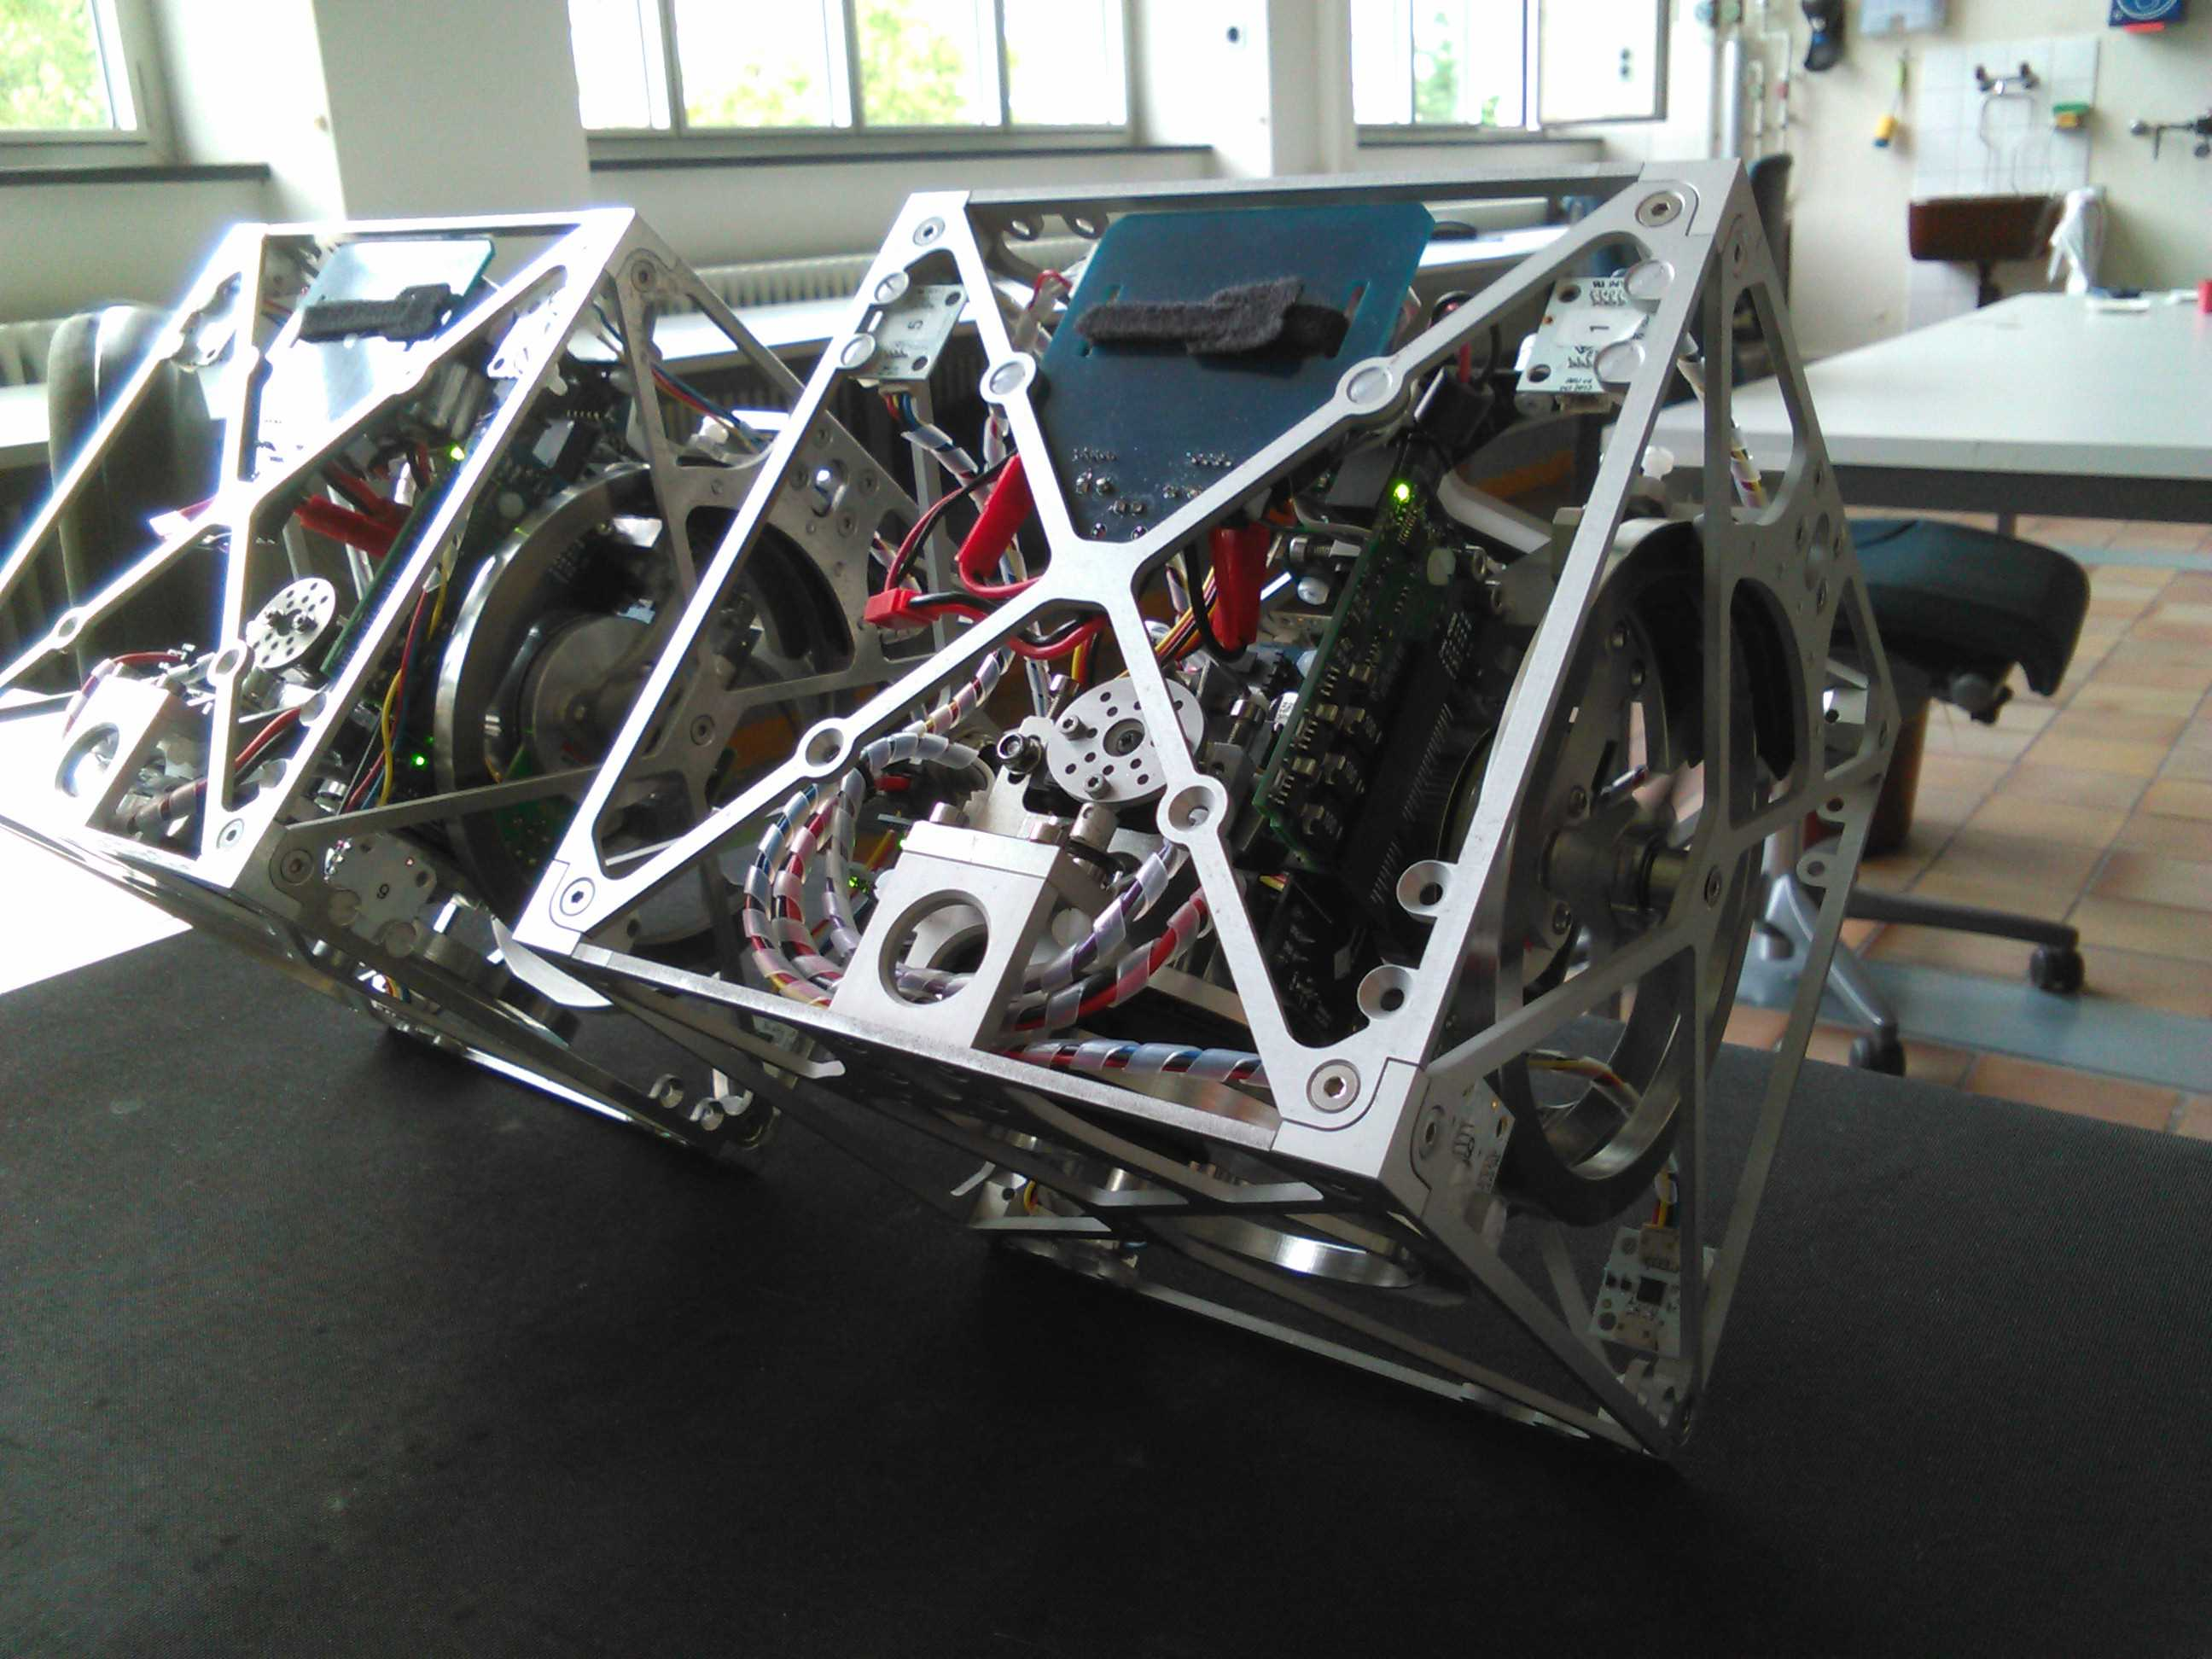
\includegraphics[width=1\textwidth]{img/Performing.jpg}
   \caption{Two Cublis jumping in sync during a choreography in the IDSC lab.}
   \label{img:performing}
\end{figure}

Much has been learnt in the process, and it is hoped that the efforts to augment Cubli continue after the completion of this project.

\section{What's next}

This project having reached its end, the outlook towards future Cubli possibilities is optimistic. Each conceptual goal developed, and fulfilled, has created potential avenues of innovation, and inspired ideas for future work on making Cubli an ever more capable robot.\\

A few examples which could be considered promising are detailed here:

\begin{itemize}
\item Jumping from any face/slanted position. Though this would require a more general approach in the controller tasks, it would allow Cubli to be independent from human intervention in almost all movement scenarios. It is estimated that the main necessary steps to undertake in order to implement this capability are : - outlining current face, edge, or corner based on IMU measurements. - use an angle system-state which is normalized to the current face.

\item Very little computer intervention - interactive Cublis. The main obstacle to overcome in order to achieve this capability is the communications failure rate. Barring that, emphasis can  be made on communications between Cublis rather than between Cubli and computer. The code developed during this project has generally been designed to enable the future implementation of these abilities.

\item Defining not just actions but movements ( go from A to B, head towards Cubli 1, ... ). Also an augmentation of Cubli intelligence, the algorithms necessary to adapt cube movements and resulting changes of coordinate systems into broader actions would certainly be interesting to develop. Resulting behavior could open up the door to new possibilities especially  if combined with the other examples presented here.

\end{itemize}

\section{Acknowledgements}

Thanks go to the IDSC team, for all the help in the face of difficulties, bugs, computer whims, and challenges.

\cleardoublepage

% Remove this:
\chapter{Working with \LaTeX\ }\label{sec:working}
This chapter explains how to typeset some of the most common elements contained in a technical report using \LaTeX.

\section{Headings}
Your report can be structured using several different types of headings. Use the commands \texttt{\textbackslash chapter\{.\}}, \texttt{\textbackslash section\{.\}}, \texttt{\textbackslash subsection\{.\}}, and \texttt{\textbackslash subsubsection\{.\}}. Use the asterisk symbol \texttt{*} to suppress numbering of a certain heading if necessary, for example, \texttt{\textbackslash section*\{.\}}.

\section{References and Footnotes}\label{sec:references}
References to literature are included using the command \texttt{\textbackslash
cite\{.\}}. For example . Your references must be entered in the file \texttt{bibliography.bib}. Making changes or adding new references in the bibliography file can be done manually or by using specialized software such as \textit{JabRef} which is free of charge.
 
Cross-referencing within the text is easily done using \texttt{\textbackslash label\{.\}} and \texttt{\textbackslash ref\{.\}}. For example, this paragraph is part of chapter~\ref{sec:working}; more specifically section~\ref{sec:references} on page~\pageref{sec:references}. You will need to compile your document twice in order for the cross-referencing to be updated.

Footnotes\footnote{The use of footnotes is generally not recommended.} are added using the command \texttt{\textbackslash footnote\{.\}}, but try to avoid the used of footnotes altogether.

\section{Lists}\label{sec:lists}
Three types of list-environments are commonly used: \texttt{itemize}, \texttt{enumerate}, and \texttt{description}. The following example uses \texttt{itemize} to create a list without numbering
\begin{itemize}
  \item point one; and
  \item point two
\end{itemize}
created using
\begin{verbatim}
\begin{itemize}
  \item point one; and
  \item point two
\end{itemize}
\end{verbatim}

The following example uses \texttt{enumerate} to create a list with numbering
\begin{enumerate}
  \item point one; and
  \item point two
\end{enumerate}
created using
\begin{verbatim}
\begin{enumerate}
  \item point one; and
  \item point two
\end{enumerate}
\end{verbatim}

The following example uses \texttt{description} to create a list with custom text as bullet-points
\begin{description}
  \item[P1] point one; and
  \item[P2] point two
\end{description}
created using
\begin{verbatim}
\begin{description}
  \item[P1] point one; and
  \item[P2] point two
\end{description}
\end{verbatim}


\section{Tables}\label{sec:tables}
Table~\ref{tab:table} shows an example of a simple table-layout. Try to avoid vertical lines on tables. The Internet contains countless resources on how to create special elements and structures in tables such as cells spanning multiple rows, rotated text, sideways tables, justification of cell elements, etc.
\begin{table}[ht]
\begin{center}
\caption{Driving cycle data of ECE-15, EUDC, and NEDC.}\vspace{1ex}
\label{tab:table}
\begin{tabular}{llccc}\hline
Description & Unit & ECE & EUDC & NEDC \\ \hline
Duration & s & 780 & 400 & 1180 \\
Distance & km & 4.052 & 6.955 & 11.007 \\
Average velocity & km/h & 18.7 &  62.6 & 33.6 \\
Idle speed & \% & 36 & 10 & 27 \\ \hline
\end{tabular}
\end{center}
\end{table}

This table was created using
\begin{verbatim}
\begin{table}[ht]
\begin{center}
\caption{Driving cycle data of ECE-15, EUDC, and NEDC.}\vspace{1ex}
\label{tab:table}
\begin{tabular}{llccc}\hline
Description & Unit & ECE & EUDC & NEDC \\ \hline
Duration & s & 780 & 400 & 1180 \\
Distance & km & 4.052 & 6.955 & 11.007 \\
Average velocity & km/h & 18.7 &  62.6 & 33.6 \\
Idle speed & \% & 36 & 10 & 27 \\ \hline
\end{tabular}
\end{center}
\end{table}
\end{verbatim}
Table~\ref{tab:table_advanced} shows a more advanced version of Tab.~\ref{tab:table} using the \texttt{booktabs} package. Inspect the source code of this document to see how this was done.
\begin{table}[ht]
\begin{center}
\small
\caption{Driving cycle data of ECE-15, EUDC, and NEDC.}\vspace{1ex}
\label{tab:table_advanced}
\begin{tabular}{@{}lcccc@{}}\toprule[1.5pt]
& & \multicolumn{3}{c}{\bf Driving cycle}\\
\cmidrule{3-5}
Description & Unit & {ECE} & {EUDC} & {NEDC} \\ \midrule
Duration & \unit[]{s} & 780 & 400 & 1180 \\
Distance & \unit[]{km} & 4.052 & 6.955 & 11.007 \\
Average velocity & \unitfrac[]{km}{h} & 18.7 &  62.6 & 33.6 \\
Idle speed & \unit[]{\%} & 36 & 10 & 27 \\ \bottomrule[1.5pt]
\end{tabular}
\end{center}
\end{table}



\section{Working with Units}
The package \texttt{\textbackslash usepackage\{units\}} enables two useful commands, namely \texttt{\textbackslash unit[.]\{.\}} and \\ \texttt{\textbackslash unitfrac[.]\{.\}\{.\}}. Use these commands to display units in a concise way, for example
\begin{align}
\delta t &= \unit[1]{s}\\
v &= \unitfrac[5]{m}{s}.
\end{align}
This example was done using
\begin{verbatim}
\begin{align}
\delta t &= \unit[1]{s}\\
v &= \unitfrac[5]{m}{s}.
\end{align}
\end{verbatim}

\section{Including Graphics}\label{sec:epsgraph}
It is recommended that you only use encapsulated post-script graphics \texttt{.eps} in your report. If you mix \texttt{.eps} with other formats such as \texttt{.png}, \texttt{.jpeg} or \texttt{.gif}, you will most likely not be able to compile your report without errors. Note that figures created in \textsc{Matlab} are easily saved in \texttt{.eps} format.

The inclusion of a figure can be done in the following way:
\begin{verbatim}
\begin{figure}[ht]
   \centering
   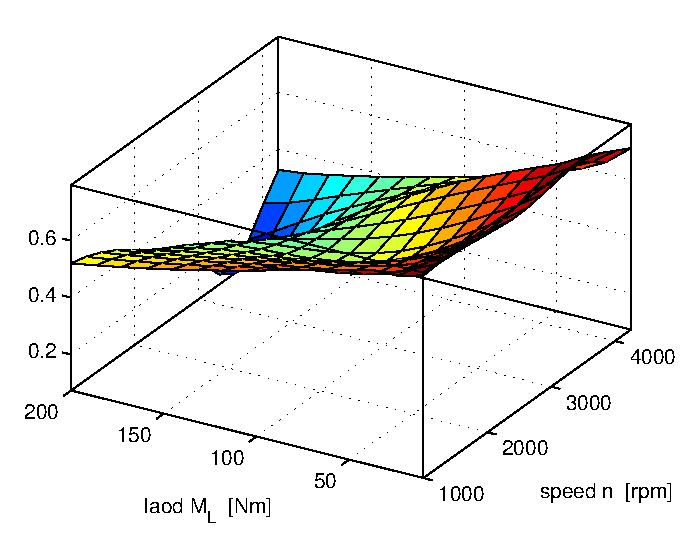
\includegraphics[width=0.75\textwidth]{img/k_surf.eps}
   \caption{Example of a figure.}
   \label{img:k_surf}
\end{figure}
\end{verbatim}

\begin{figure}[ht]
   \centering
   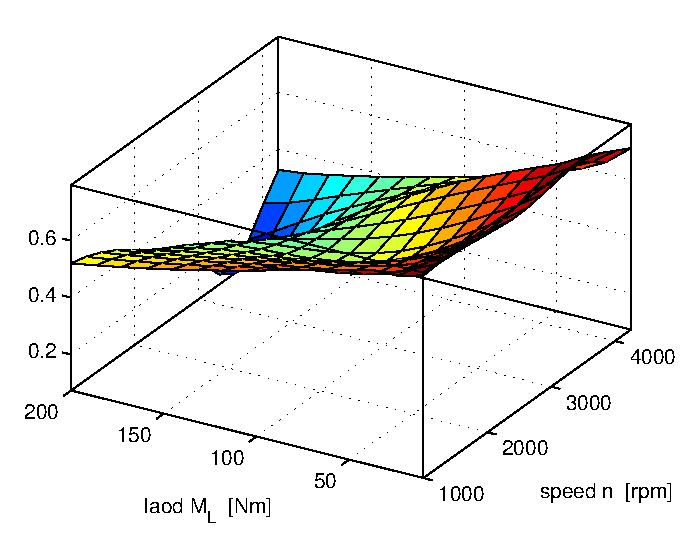
\includegraphics[width=0.75\textwidth]{img/k_surf.eps}
   \caption{Example of a figure.}
   \label{img:k_surf}
\end{figure}

Two figures are displayed next to each other using
\begin{verbatim}
\begin{figure}[ht]
  \begin{minipage}[t]{0.48\textwidth}
    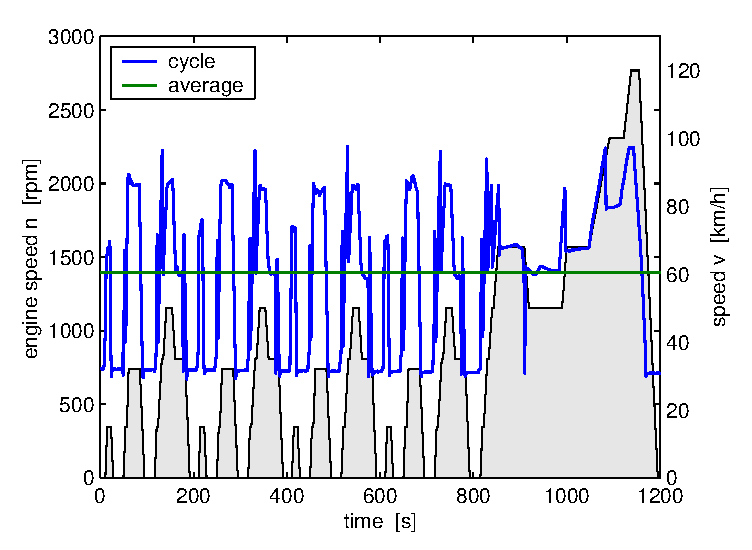
\includegraphics[width = \textwidth]{img/cycle_we.eps}
  \end{minipage}
  \hfill
  \begin{minipage}[t]{0.48\textwidth}
    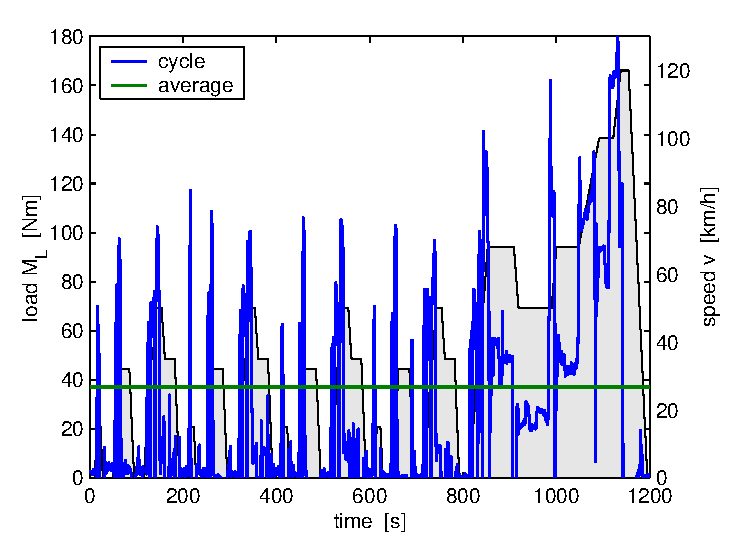
\includegraphics[width = \textwidth]{img/cycle_ml.eps}
  \end{minipage}
  \caption{Two figures next to each other.}
  \label{img:cycle}
\end{figure}
\end{verbatim}

\begin{figure}[ht]
  \begin{minipage}[t]{0.48\textwidth}
    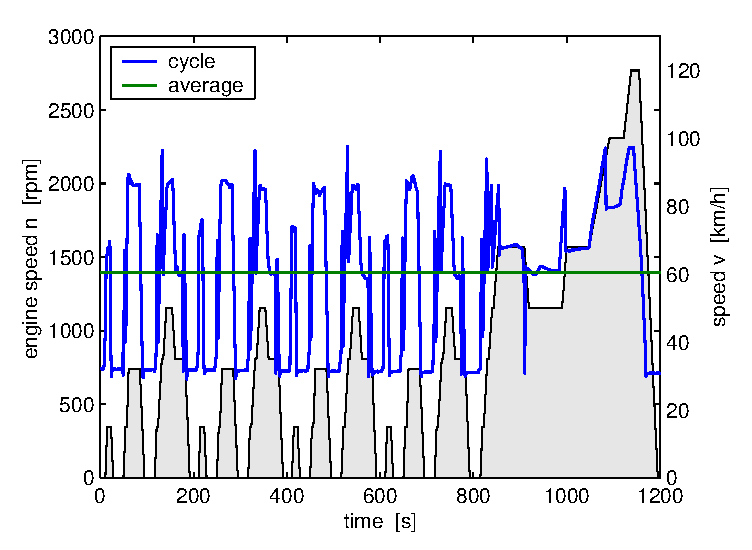
\includegraphics[width = \textwidth]{img/cycle_we.eps}
  \end{minipage}
  \hfill
  \begin{minipage}[t]{0.48\textwidth}
    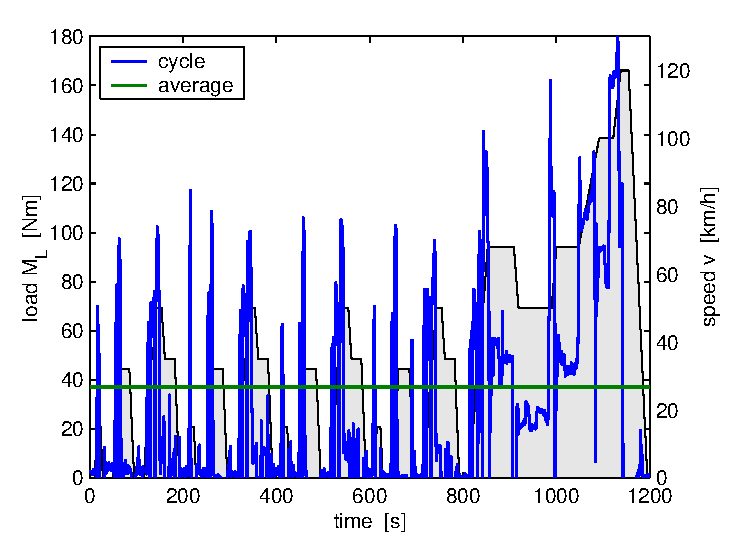
\includegraphics[width = \textwidth]{img/cycle_ml.eps}
  \end{minipage}
  \caption{Two figures next to each other.}
  \label{img:cycle}
\end{figure}

The positioning parameter \texttt{h} (here) forces your figure to be placed in the current position relative to your text. You may add \texttt{t} (top), \texttt{b} (bottom), and/or \texttt{p} (page) to allow for more flexible positioning within your document. For instance, \texttt{[tb]} forces your figure to be placed either on the top or bottom of a page.


\section{Equations}\label{sec:math}
The most common way to include equations is using the \texttt{equation} environment.
\begin{equation}\label{eq:p_me0f}
 p_\mathrm{me0f}(T_e,\omega_e) \ = \ k_1(T_e) \cdot (k_2+k_3 S^2
 \omega_e^2) \cdot \Pi_\mathrm{max} \cdot \sqrt{\frac{k_4}{B}} \, .
\end{equation}
It is recommended to use \texttt{\textbackslash mathrm\{.\}} for subscripts comprising more than two letters since it reduces the width of the subscript significantly and improves readability. The corresponding code is
\begin{verbatim}
\begin{equation}\label{eq:p_me0f}
 p_\mathrm{me0f}(T_e,\omega_e) \ = \ k_1(T_e) \cdot (k_2+k_3 S^2
 \omega_e^2) \cdot \Pi_\mathrm{max} \cdot \sqrt{\frac{k_4}{B}} \, .
\end{equation}
\end{verbatim}
Equations, such as Eq.~\eqref{eq:p_me0f}, may be referenced using \texttt{\textbackslash eqref\{.\}}. In-line mathematical content is created using \texttt{\$.\$}, for example $a^2+b^2=c^2$. It is practically possible to typeset any equation in \LaTeX. Equation~\eqref{eq:advanced} shows an example of a more advance structure.
\begin{equation}\label{eq:advanced}
x^k_n(i) = \left\{\begin{array}{ll}y(i) & \text{if}\quad x^k_{n-1}(i)\leq \mathbf{x}\\
z(i) & \text{otherwise}\end{array}\right., \text{for}\quad i=\{1,\ldots,N\}.
\end{equation}



\section{Including Code in your Document}
Include samples from your Matlab code using the \texttt{lstlistings} environment, for example
\lstset{language=Matlab,numbers=none}
\begin{lstlisting}[frame=lines]
% Evaluate y = 2x
for i = 1:length(x)

  y(i) = 2*x(i);

end
\end{lstlisting}
This example was created using
\begin{verbatim}
\lstset{language=Matlab,numbers=none}
\begin{lstlisting}[frame=lines]
% Evaluate y = 2x
for i = 1:length(x)

  y(i) = 2*x(i);

end
\end{lstlisting}
\end{verbatim}
where \texttt{\textbackslash usepackage\{mcode\}} must be included in the preamble of your document. If you want to include the entire content of a file \texttt{mycode.m} in your document, simply input the path to \texttt{mycode.m} instead of pasting the entire content into your \TeX -file
\begin{verbatim}
\lstset{language=Matlab,numbers=left}
\lstinputlisting{path/to/mycode.m}
\end{verbatim}
Including the path to your m-file also ensures that the code in your report is always up-to-date. The \texttt{\textbackslash lstset\{language=Matlab\}} command ensures that \textsc{Matlab} syntax definitions are used, but many other languages are recognised as well such as \texttt{Fortran} and \texttt{C++}.
\cleardoublepage

% Appendix______________________________________________________________________
\appendix
\chapter{Bugs and Issues}\label{sec:bugsandissues}

It is said that one learns more from what goes wrong than from what goes well. As such this section is written in the hope that future readers might  
\begin{itemize}
\item[a.] Learn something interesting about peculiarities in the concerned systems
\item[b.] Deepen their understanding of the edge cases emerging from current implementation  
\item[c.]Avoid repeating similar mistakes 
\end{itemize}
 
\section{Hash Incompatibility}

\textbf{Symptoms:} same code compiled on both machines, but neither accepts each other's messages.\\
Although both machines could be shown to transmit and receive the full messages correctly. Messages were not decrypted successfully. The error was raised that hashes were not in accordance, even though all the hash generation/checking code was compiled from the same source, the shared com\_protocol.c file, in both modules. This was due to an oversight in typecasting from signed values to unsigned value, resulting in potentially compiler-dependent behavior. \\
For example: 1-byte signed char 11111000 to unsigned 2 byte int becomes either 11111111 11111000 or 00000000 11111000 depending on the compiler. One being significantly larger than the other.  \\
\textbf{Note:} All data transmitted through the serial port is necessarily converted to chars ( 8 bit values ), with existing Cubli code using specifically signed chars. On the other hand some mathematical and shift operations are fully defined only on unsigned variables. Be knowledgeable or test extensively when converting from one to the other.  
 
\section{Unstable behavior when Cubli doesn't have a fall-to-face delay} 

 \cleardoublepage


\chapter{Again Something}\label{sec:again_something}

Blah, blah \dots

 \cleardoublepage



% Bibliography__________________________________________________________________
% Literature (Additional references can be added to the .bib-file manually, or by using, for example, the free application JabRef). Compile in the following order: latex -bibtex -latex -latex

\bibliographystyle{plain}
\bibliography{bibliography}

\end{document}